% $Header$

\documentclass[aspectratio=43,dvipsnames,usenames, svgnames]{beamer}

\mode<presentation>
{
  \usetheme{CambridgeUS}
%  \usetheme{Boadilla}
  \usecolortheme{dolphin}
%  \usecolortheme{albatross}
  \useinnertheme{circles}
  \setbeamercovered{transparent}
}
\usefonttheme[onlymath]{serif}  % article math
\usepackage[english]{babel}
\usepackage{ulem}
\usepackage{booktabs}
\usepackage{tabularx, colortbl}
\usepackage{amssymb}
\usepackage{tikz}
\usetikzlibrary{calc, shapes.callouts}
\usepackage{tikzpeople}
\usepackage{graphicx}
\usepackage{xcolor}
\usepackage[latin1]{inputenc}
\usepackage{times}
\usepackage[T1]{fontenc}
% Or whatever. Note that the encoding and the font should match. If T1
% does not look nice, try deleting the line with the fontenc.
\usepackage{mathrsfs}
\newtheorem{assumption}{Assumption}
%\newtheorem{corollary}{Corollary}
%\newfont {\aaa} {msbm10 scaled \megstep 0}
\usepackage{bm}
\usepackage{subfigure, graphicx}
\usepackage{multirow, booktabs}
\usepackage{pstricks}
\usepackage[customcolors]{hf-tikz}
%\graphicspath{{images/}}

\title[Systemic Risk: Cross Section] % (optional, use only with long paper titles)
{Systemic Risk:\\ the Cross-Section Dimension}

\author[Chan-Lau (IMF and NUS)] % (optional, use only with lots of authors)
{\normalsize{Jorge A. Chan-Lau}\\
\scriptsize{\url{jchanlau@imf.org}}}
% - Give the names in the same order as the appear in the paper.
% - Use the \inst{?} command only if the authors have different
%   affiliation.

\institute[] % (optional, but mostly needed)
{\footnotesize{
  Institute for Capacity and Development, International Monetary Fund \\
  Credit Research Initiative, National University of Singapore
  }}
% - Use the \inst command only if there are several affiliations.
% - Keep it simple, no one is interested in your street address.

\date[November 2017] % (optional, should be abbreviation of conference name)
{\footnotesize{Structured Curriculum Course\\
Macrofinancial Linkages, Systemic Risk, and Macroprudential policy}
\vspace{1em}

{\footnotesize{International Monetary Fund\\
November 6-8, 2017, Washington, D.C.\\}}

\vspace{1em}
\tiny{Do not reproduce or re-distribute without permission}
}
% - Either use conference name or its abbreviation.
% - Not really informative to the audience, more for people (including
%   yourself) who are reading the slides online


% If you have a file called "university-logo-filename.xxx", where xxx
% is a graphic format that can be processed by latex or pdflatex,
% resp., then you can add a logo as follows:

% \pgfdeclareimage[height=0.5cm]{university-logo}{university-logo-filename}
% \logo{\pgfuseimage{university-logo}}

% Delete this, if you do not want the table of contents to pop up at
% the beginning of each subsection:
%\AtBeginSubSection[]
%{
%  \begin{frame}<beamer>{Outline}
%    \tableofcontents[currentsection]
%  \end{frame}
%}

\AtBeginSection[]
{
  \begin{frame}
  \frametitle{Outline}
	  \tableofcontents[
	  currentsection,
	  sectionstyle=show/shaded,
	  subsectionstyle=show/show/hide
	  ]
  \end{frame}
}

% If you wish to uncover everything in a step-wise fashion, uncomment
% the following command: 

%\beamerdefaultoverlayspecification{<+->}

\graphicspath{{figures/}}

\begin{document}
\begin{frame} % Titlepage creation
  \titlepage
\end{frame}
\begin{frame}{Outline} % Outline creation
  \tableofcontents[hideallsubsections]
  % You might wish to add the option [pausesections]
\end{frame}

\begin{frame} % Key Learning Points (1)
\frametitle{Key Learning Points (1)}
\begin{itemize}
	\item Conceptual Overview
		\begin{itemize}
			\item Interconnectedness
			\item Systemic risk
		\end{itemize}
	\smallskip
	\item From Concept to Practice
		\begin{itemize}
			\item Direct exposure networks
			\smallskip
			\item Market-based networks
			\smallskip
			\item Portfolio Approaches
		\end{itemize}
	\end{itemize}
\end{frame}

\begin{frame} % Key Learning Points (2)
\frametitle{Key Learning Points (2)}
\begin{itemize}
	\item What practical people do
		\begin{itemize}
			\item Indicator approach for G-SIBs
		\end{itemize}
	\smallskip
	\item New directions
		\begin{itemize}
			\item Systemic communities
			\item Agent-based models
		\end{itemize}
	\smallskip
	\item Hands-on exercises
		\begin{itemize}
			\item Direct exposure networks (Excel)
			\item CoVaR - CoRisk calculations
			\item Portfolio approach
		\end{itemize}
\end{itemize}
\end{frame}

\section{Conceptual overview}

\subsection{Interconnectedness and systemic risk}

\begin{frame} % Interconnectedness and Systemic Risk
\frametitle{Interconnectedness and systemic risk}
	\begin{itemize}
		\item Structure of financial system
		\begin{itemize}
			\item Direct exposures
			\item Common exposures
		\end{itemize}
		\smallskip	
		\item Interconnectedness (cross-section) 
		\begin{itemize}
			\item Contagion and shock amplification
			\item Domino effects
			\item Adverse spillovers
		\end{itemize}
	\end{itemize}
\end{frame}

\begin{frame} % Liquidity spiral: example cross-sectional risk
\frametitle{Liquidity spiral: a systemic risk manifestation}
\begin{center}
	\includegraphics[scale=0.52]{figures/figLiquiditySpiral.eps}
\end{center}
\tiny{Source: Brunnermeier and Pedersen (2009)}
\end{frame}

\subsection{Financial systems as networks}

\begin{frame} % Financial systems as networks
\begin{center}
	\Large{Financial systems as networks}
\end{center}
\end{frame}

\begin{frame} % Network representation
\frametitle{Network representation}
\begin{itemize}
	\item Networks serve to visualize and to analyze interconnectedness
	\smallskip
	\item Networks has two main elements
	\begin{itemize}
		\item Nodes (vertices)
		\item Edges (links)
	\end{itemize}
	\smallskip
	\item Nodes
	\begin{itemize}
		\item Firms
		\item Markets
		\item Risk factors
	\end{itemize}
	\smallskip
	\item Edges
	\begin{itemize}
		\item Inter-firm loans
		\item Security price correlations
		\item Spillover measures
	\end{itemize}
\end{itemize}
\end{frame}

\begin{frame} % Interfirm exposures (1)
\frametitle{Interfirm exposures (1)}
\begin{center}
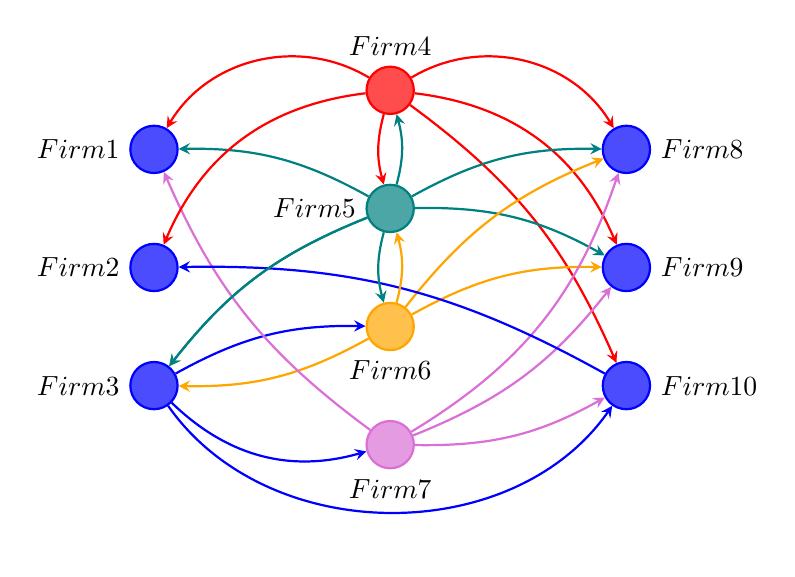
\begin{tikzpicture}
	[firm/.style={circle,draw=blue, fill=blue!70, thick,
				   inner sep=0pt, minimum size=6mm},
	 risk/.style={circle, inner sep=0pt, minimum size=6mm}]
	\node at (0,0)    [risk,draw=Orchid, fill=Orchid!70, thick](rf4)
					  [label=below:$\text{Firm }7$]{};
	\node at (0,1.5)  [risk,draw=Orange, fill=Orange!70,thick](rf3)
	                  [label=below:$\text{Firm }6$]{};
	\node at (0,3.0)  [risk,draw=teal, fill=teal!70, thick](rf2)
				   	  [label=left:$\text{Firm }5$]{};
	\node at (0,4.5)  [risk,draw=red, fill=red!70, thick](rf1)
	                  [label=above:$\text{Firm }4$]{};
	\node at (3,0.75) [firm](fm10)[label=right:$\text{Firm }10$]{};	
	\node at (3,2.25) [firm](fm9)[label=right:$\text{Firm }9$]{};	
	\node at (3,3.75) [firm](fm8)[label=right:$\text{Firm }8$]{};	
	\node at (-3,0.75) [firm](fm3)[label=left:$\text{Firm }3$]{};	
	\node at (-3,2.25) [firm](fm2)[label=left:$\text{Firm }2$]{};	
	\node at (-3,3.75) [firm](fm1)[label=left:$\text{Firm }1$]{};	
	\draw[-stealth,red,thick]    (rf1) to [bend left = 45](fm8);
	\draw[-stealth,red,thick]    (rf1) to [bend left = 30](fm9);
	\draw[-stealth,red,thick]    (rf1) to [bend left = 15](fm10);	
	\draw[-stealth,teal,thick]   (rf2) to [bend left = 15](fm8);
	\draw[-stealth,teal,thick]   (rf2) to [bend left = 15](fm9);
	\draw[-stealth,Orange,thick] (rf3) to [bend left = 15](fm8);
	\draw[-stealth,Orange,thick] (rf3) to [bend left = 15](fm9);		
	\draw[-stealth,Orchid,thick] (rf4) to [bend right = 20](fm8);
	\draw[-stealth,Orchid,thick] (rf4) to [bend right = 15](fm9);
	\draw[-stealth,Orchid,thick] (rf4) to [bend right = 15](fm10);	
	\draw[-stealth,Orange,thick] (rf3) to [bend left = 15](fm3);
	\draw[-stealth,blue,thick]   (fm3) to [bend left = 15](rf3);
	\draw[-stealth,blue,thick]   (fm3) to [bend right = 30](rf4);	
	\draw[-stealth,Orchid,thick] (rf4) to [bend left = 15](fm1);	
	\draw[-stealth,blue,thick]   (fm3) to [bend left = -55](fm10);	
	\draw[-stealth,blue,thick]   (fm10) to [bend right = 15](fm2);	
	\draw[-stealth,teal,thick]   (rf2) to [bend right = 15](fm1);
	\draw[-stealth,teal,thick]   (rf2) to [bend right = 15](fm3);
	\draw[-stealth,red,thick]    (rf1) to [bend right = 45](fm1);
	\draw[-stealth,red,thick]    (rf1) to [bend right = 30](fm2);
	\draw[-stealth,teal,thick]   (rf2) to [bend right = 15](fm3);
	\draw[-stealth,Orange,thick] (rf3) to [bend right = 15](rf2);			
	\draw[-stealth,Teal,thick] (rf2) to [bend right = 15](rf1);				
	\draw[-stealth,Teal,thick] (rf2) to [bend right = 15](rf3);					
	\draw[-stealth,red,thick] (rf1) to [bend right = 15](rf2);					
\end{tikzpicture}
\end{center}
\end{frame}

\begin{frame} % Interfirm exposures (2)
\frametitle{Interfirm exposures (2)}
\begin{center}
	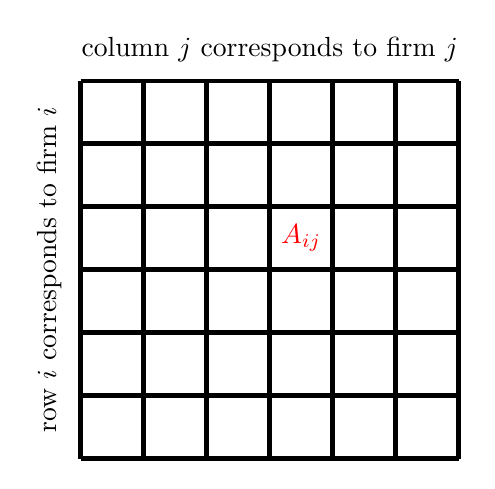
\begin{tikzpicture}
		\draw[step=0.8cm, ultra thick] (0,0) grid (6*0.8,6*0.8);
		\node[color=red,thick] at (3.5*0.8,3.5*0.8){$A_{ij}$};
		\node at (3*0.8,6.5*0.8){column $j$ corresponds to firm $j$};
		\node[rotate=90] at (-0.5*0.8,3*0.8) {row $i$ corresponds to firm $i$};
	\end{tikzpicture}
\end{center}
\begin{center}
$A_{ij}$ is claim of firm $i$ on firm $j$
\end{center}
\end{frame}

\begin{frame} % Exposures to common factors (1)
\frametitle{Exposure to common factors (1)}
\begin{center}
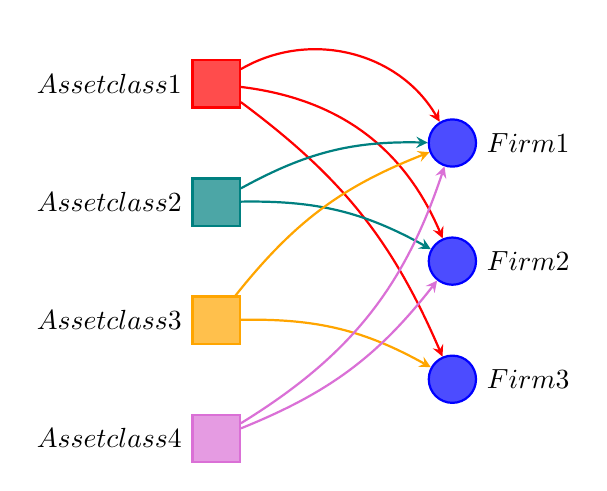
\begin{tikzpicture}
	[firm/.style={circle,draw=blue, fill=blue!70, thick,
				   inner sep=0pt, minimum size=6mm},
	 risk/.style={rectangle, inner sep=0pt, minimum size=6mm}]
	\node at (0,0)    [risk,draw=Orchid, fill=Orchid!70, thick](rf4)
					  [label=left:$\text{Asset class }4$]{};
	\node at (0,1.5)  [risk,draw=Orange, fill=Orange!70,thick](rf3)
	                  [label=left:$\text{Asset class }3$]{};
	\node at (0,3.0)  [risk,draw=teal, fill=teal!70, thick](rf2)
				   	  [label=left:$\text{Asset class }2$]{};
	\node at (0,4.5)  [risk,draw=red, fill=red!70, thick](rf1)
	                  [label=left:$\text{Asset class }1$]{};
	\node at (3,0.75) [firm](fm3)[label=right:$\text{Firm }3$]{};	
	\node at (3,2.25) [firm](fm2)[label=right:$\text{Firm }2$]{};	
	\node at (3,3.75) [firm](fm1)[label=right:$\text{Firm }1$]{};	
	\draw[-stealth,red,thick]    (rf1) to [bend left = 45](fm1);
	\draw[-stealth,red,thick]    (rf1) to [bend left = 30](fm2);
	\draw[-stealth,red,thick]    (rf1) to [bend left = 15](fm3);	
	\draw[-stealth,teal,thick]   (rf2) to [bend left = 15](fm1);
	\draw[-stealth,teal,thick]   (rf2) to [bend left = 15](fm2);
	\draw[-stealth,Orange,thick]   (rf3) to [bend left = 15](fm1);
	\draw[-stealth,Orange,thick]   (rf3) to [bend left = 15](fm3);		
	\draw[-stealth,Orchid,thick] (rf4) to [bend right = 20](fm1);
	\draw[-stealth,Orchid,thick] (rf4) to [bend right = 15](fm2);
\end{tikzpicture}
\end{center}
\begin{flushleft}
\scriptsize{* This is a bipartite network, e.g. Zhao et al (2013)}
\end{flushleft}
\end{frame}

\begin{frame} % Exposure to common factors (2)
\frametitle{Exposure to common factors (2)}
\begin{center}
	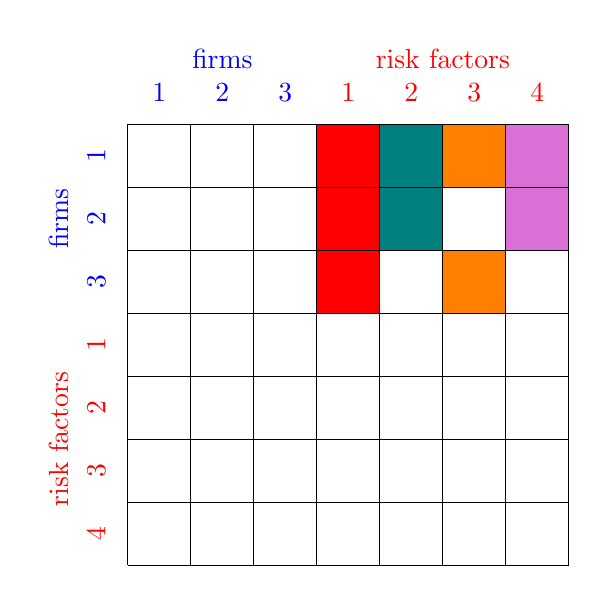
\begin{tikzpicture}
	[every node/.style={minimum size=.8cm-\pgflinewidth}]
		\draw[step=0.8cm,color=black] (0,0) grid (7*0.8,7*0.8);
		\node[color=red] at (5*0.8,1.005*8*0.8){risk factors};
		\node[color=red] at (3.5*0.8, 7.5*0.8){1};				
		\node[color=red] at (4.5*0.8, 7.5*0.8){2};		
		\node[color=red] at (5.5*0.8, 7.5*0.8){3};		
		\node[color=red] at (6.5*0.8, 7.5*0.8){4};				
		\node[color=blue] at (1.5*0.8, 1.005*8*0.8){firms};
		\node[color=blue] at (0.5*0.8, 7.5*0.8){1};				
		\node[color=blue] at (1.5*0.8, 7.5*0.8){2};				
		\node[color=blue] at (2.5*0.8, 7.5*0.8){3};						
		\node[rotate=90, color =red] at (-1.1*0.8,2*0.8) {risk factors};
		\node[rotate=90, color =red] at (-0.5*0.8,0.5*0.8) {4};
		\node[rotate=90, color =red] at (-0.5*0.8,1.5*0.8) {3};
		\node[rotate=90, color =red] at (-0.5*0.8,2.5*0.8) {2};				
		\node[rotate=90, color =red] at (-0.5*0.8,3.5*0.8) {1};	
		\node[rotate=90, color =blue]at (-1.1*0.8,5.5*0.8){firms};
		\node[rotate=90, color =blue] at (-0.5*0.8,4.5*0.8) {3};
		\node[rotate=90, color =blue] at (-0.5*0.8,5.5*0.8) {2};				
		\node[rotate=90, color =blue] at (-0.5*0.8,6.5*0.8) {1};				
		\node[fill=red] at (3.5*0.8,6.5*0.8){};
		\node[fill=teal] at (4.5*0.8,6.5*0.8){};
		\node[fill=orange] at (5.5*0.8,6.5*0.8){};		
		\node[fill=Orchid] at (6.5*0.8,6.5*0.8){};				
		\node[fill=red] at (3.5*0.8,5.5*0.8){};
		\node[fill=teal] at (4.5*0.8,5.5*0.8){};
%		\node[fill=orange] at (5.5*0.8,5.5*0.8){};		
		\node[fill=Orchid] at (6.5*0.8,5.5*0.8){};				
		\node[fill=red] at (3.5*0.8,4.5*0.8){};
%		\node[fill=teal] at (4.5*0.8,4.5*0.8){};
		\node[fill=orange] at (5.5*0.8,4.5*0.8){};		
%		\node[fill=red] at (6.5*0.8,4.5*0.8){};				
	\end{tikzpicture}
\end{center}
\end{frame}

\begin{frame} % Interfirm and common factor exposures
\frametitle{Interfirm and common factor exposures}
\begin{center}
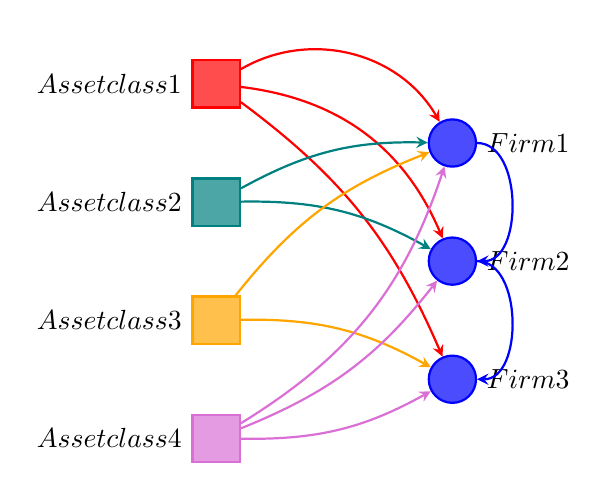
\begin{tikzpicture}
	[firm/.style={circle,draw=blue, fill=blue!70, thick,
				   inner sep=0pt, minimum size=6mm},
	 risk/.style={rectangle, inner sep=0pt, minimum size=6mm}]
	\node at (0,0)    [risk,draw=Orchid, fill=Orchid!70, thick](rf4)
					  [label=left:$\text{Asset class }4$]{};
	\node at (0,1.5)  [risk,draw=Orange, fill=Orange!70,thick](rf3)
	                  [label=left:$\text{Asset class }3$]{};
	\node at (0,3.0)  [risk,draw=teal, fill=teal!70, thick](rf2)
				   	  [label=left:$\text{Asset class }2$]{};
	\node at (0,4.5)  [risk,draw=red, fill=red!70, thick](rf1)
	                  [label=left:$\text{Asset class }1$]{};
	\node at (3,0.75) [firm](fm3)[label=right:$\text{      Firm }3$]{};	
	\node at (3,2.25) [firm](fm2)[label=right:$\text{      Firm }2$]{};	
	\node at (3,3.75) [firm](fm1)[label=right:$\text{      Firm }1$]{};	
	\draw[-stealth,red,thick]    (rf1) to [bend left = 45](fm1);
	\draw[-stealth,red,thick]    (rf1) to [bend left = 30](fm2);
	\draw[-stealth,red,thick]    (rf1) to [bend left = 15](fm3);	
	\draw[-stealth,teal,thick]   (rf2) to [bend left = 15](fm1);
	\draw[-stealth,teal,thick]   (rf2) to [bend left = 15](fm2);
	\draw[-stealth,Orange,thick] (rf3) to [bend left = 15](fm1);
	\draw[-stealth,Orange,thick] (rf3) to [bend left = 15](fm3);		
	\draw[-stealth,Orchid,thick] (rf4) to [bend right = 20](fm1);
	\draw[-stealth,Orchid,thick] (rf4) to [bend right = 15](fm2);
	\draw[-stealth,Orchid,thick] (rf4) to [bend right = 15](fm3);	
	\draw[-stealth,blue,thick]   (fm1) to [bend right = -90](fm2);
	\draw[-stealth,blue,thick]   (fm2) to [bend right = -90](fm3);
\end{tikzpicture}
\end{center}
\end{frame}

\begin{frame} % Interfirm and common factor exposures (2)
\frametitle{Interfirm and common factors (2)}
\begin{center}
	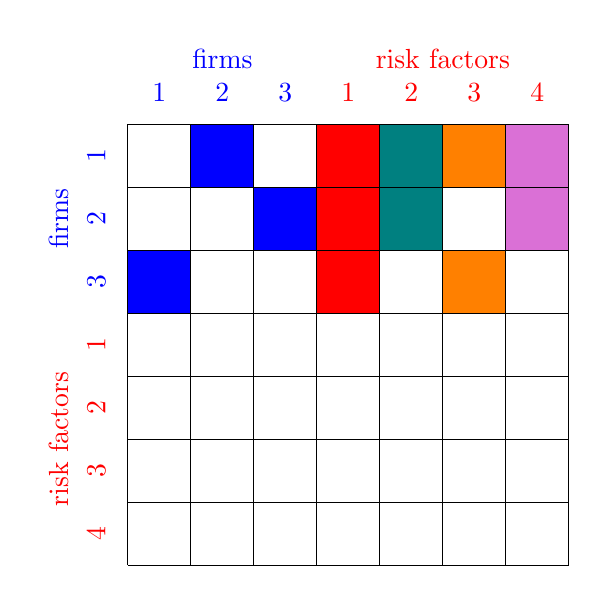
\begin{tikzpicture}
	[every node/.style={minimum size=.8cm-\pgflinewidth}]
		\draw[step=0.8cm, color=black] (0,0) grid (7*0.8,7*0.8);
		\node[color=red] at (5*0.8,1.005*8*0.8){risk factors};
		\node[color=red] at (3.5*0.8, 7.5*0.8){1};				
		\node[color=red] at (4.5*0.8, 7.5*0.8){2};		
		\node[color=red] at (5.5*0.8, 7.5*0.8){3};		
		\node[color=red] at (6.5*0.8, 7.5*0.8){4};				
		\node[color=blue] at (1.5*0.8, 1.005*8*0.8){firms};
		\node[color=blue] at (0.5*0.8, 7.5*0.8){1};				
		\node[color=blue] at (1.5*0.8, 7.5*0.8){2};				
		\node[color=blue] at (2.5*0.8, 7.5*0.8){3};						
		\node[rotate=90, color =red] at (-1.1*0.8,2*0.8) {risk factors};
		\node[rotate=90, color =red] at (-0.5*0.8,0.5*0.8) {4};
		\node[rotate=90, color =red] at (-0.5*0.8,1.5*0.8) {3};
		\node[rotate=90, color =red] at (-0.5*0.8,2.5*0.8) {2};				
		\node[rotate=90, color =red] at (-0.5*0.8,3.5*0.8) {1};	
		\node[rotate=90, color =blue]at (-1.1*0.8,5.5*0.8){firms};
		\node[rotate=90, color =blue] at (-0.5*0.8,4.5*0.8) {3};
		\node[rotate=90, color =blue] at (-0.5*0.8,5.5*0.8) {2};				
		\node[rotate=90, color =blue] at (-0.5*0.8,6.5*0.8) {1};				
		\node[fill=red] at (3.5*0.8,6.5*0.8){};
		\node[fill=teal] at (4.5*0.8,6.5*0.8){};
		\node[fill=orange] at (5.5*0.8,6.5*0.8){};		
		\node[fill=Orchid] at (6.5*0.8,6.5*0.8){};				
		\node[fill=red] at (3.5*0.8,5.5*0.8){};
		\node[fill=teal] at (4.5*0.8,5.5*0.8){};
%		\node[fill=orange] at (5.5*0.8,5.5*0.8){};		
		\node[fill=Orchid] at (6.5*0.8,5.5*0.8){};				
		\node[fill=red] at (3.5*0.8,4.5*0.8){};
%		\node[fill=teal] at (4.5*0.8,4.5*0.8){};
		\node[fill=orange] at (5.5*0.8,4.5*0.8){};		
%		\node[fill=red] at (6.5*0.8,4.5*0.8){};				
		\node[fill=blue] at (1.5*0.8,6.5*0.8){};
		\node[fill=blue] at (2.5*0.8,5.5*0.8){};
		\node[fill=blue] at (0.5*0.8,4.5*0.8){};
	\end{tikzpicture}
\end{center}
\end{frame}

\begin{frame} % Multiplex networks (1)
\frametitle{Multiplex (multi-layer) networks (1)}
\begin{center}
	\includegraphics[scale=0.30]{figures/figMultilayer.eps}
\end{center}
\tiny{Source: Bookstaber and Kenett (2016)}
\end{frame}

\begin{frame} % Multiplex networks (2)
\frametitle{Multiplex (multi-layer) networks (2)}
\begin{center}
	\includegraphics[scale=0.3]{figures/figSunChanLauMultiplex.eps}
\end{center}
\tiny{Source: Sun and Chan-Lau (2017)}
\end{frame}

\section{Direct exposure networks}

\begin{frame} % Direct exposure networks
\frametitle{Direct exposure networks}
\begin{itemize}
	\item Network topology
	\begin{itemize}
		\item Nodes and connecting edges
		\item Transmits and amplifies shocks
		\item Changes constantly and frequently
		\item Dynamics not clearly understood
	\end{itemize}
	\smallskip
	\item Systemic risk analysis
	\begin{itemize}
		\item Centrality measures
		\smallskip
		\item Default simulation algorithms
			\begin{itemize}
				\item Take down one firm (or selected group) at a time
				\item Check impact on other firms
				\item Repeat cycle in case other firms default
			\end{itemize}
	\end{itemize}
	\smallskip
\end{itemize}
\end{frame}

\subsection{Why topology matters}

\begin{frame} % Why Topology Matters
\begin{center}
	\Large{Why topology matters}
\end{center}
\end{frame}

\begin{frame} % Example 1: No systemic firms
\frametitle{Example 1: No systemic firms}
\begin{center}
	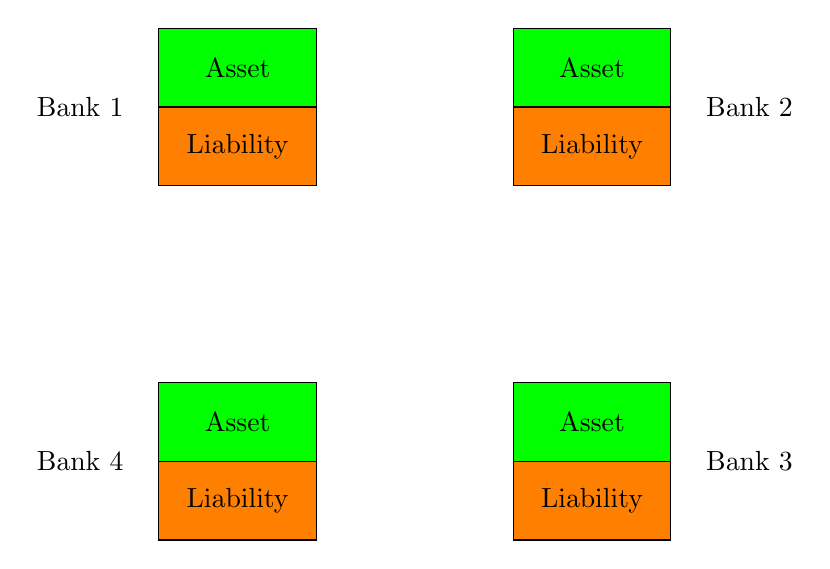
\begin{tikzpicture}
	
	    % First column
		\draw[fill=orange] (0,0) rectangle (4/2,2/2) node[pos=.5]{Liability};
		\draw[fill=green](0,2/2) rectangle (4/2,4/2) node[pos=.5]{Asset};
		\draw[fill=orange] (0,9/2) rectangle (4/2,11/2) node[pos=.5]{Liability};
		\draw[fill=green](0,11/2) rectangle (4/2,13/2)node[pos=.5]{Asset};		
		
		% Second column
		\draw[fill=orange] (9/2,0) rectangle (13/2,2/2) node[pos=.5]{Liability};
		\draw[fill=green](9/2,2/2) rectangle (13/2,4/2)node[pos=.5]{Asset};
		\draw[fill=orange] (9/2,9/2) rectangle (13/2,11/2) node[pos=.5]{Liability};
		\draw[fill=green](9/2,11/2) rectangle (13/2,13/2)node[pos=.5]{Asset};		
		
		\node at (-2/2,11/2) {Bank 1};
		\node at (15/2,11/2) {Bank 2};
		\node at (-2/2, 2/2) {Bank 4};
		\node at (15/2, 2/2) {Bank 3};
		
	\end{tikzpicture}
\end{center}
\tiny{Source: Chan-Lau (2013)}
\end{frame}

\begin{frame} % Example 2: Two systemic sub-systems
\frametitle{Example 2: Two systemic sub-systems}
\begin{center}
	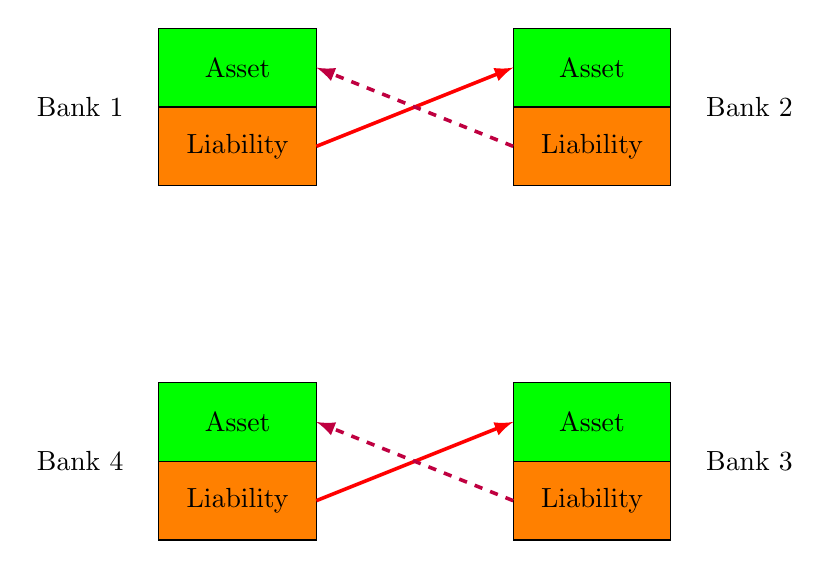
\begin{tikzpicture}
	    % First column
		\draw[fill=orange] (0,0) rectangle (4/2,2/2) node[pos=.5]{Liability};
		\draw[fill=green](0,2/2) rectangle (4/2,4/2) node[pos=.5]{Asset};
		\draw[fill=orange] (0,9/2) rectangle (4/2,11/2) node[pos=.5]{Liability};
		\draw[fill=green](0,11/2) rectangle (4/2,13/2)node[pos=.5]{Asset};		
		% Second column
		\draw[fill=orange] (9/2,0) rectangle (13/2,2/2) node[pos=.5]{Liability};
		\draw[fill=green](9/2,2/2) rectangle (13/2,4/2)node[pos=.5]{Asset};
		\draw[fill=orange] (9/2,9/2) rectangle (13/2,11/2) node[pos=.5]{Liability};
		\draw[fill=green](9/2,11/2) rectangle (13/2,13/2)node[pos=.5]{Asset};		
		% Name banks
		\node at (-2/2,11/2) {Bank 1};
		\node at (15/2,11/2) {Bank 2};
		\node at (-2/2, 2/2) {Bank 4};
		\node at (15/2, 2/2) {Bank 3};
		% Draw arrows
		\draw[-latex,red,line width=0.3ex] (4/2,10/2) -- (9/2,12/2);
		\draw[-latex,purple,dashed, line width=0.3ex] (9/2,10/2) -- (4/2,12/2);
		\draw[-latex,red,line width=0.3ex] (4/2,1/2) -- (9/2,3/2);
		\draw[-latex,purple,line width=0.3ex,dashed] (9/2,1/2) -- (4/2,3/2);
	\end{tikzpicture}
\end{center}
\tiny{Source: Chan-Lau (2013)}
\end{frame}

\begin{frame} % Example 3: One systemic firm
\frametitle{Example 3: One systemic firm}
\begin{center}
	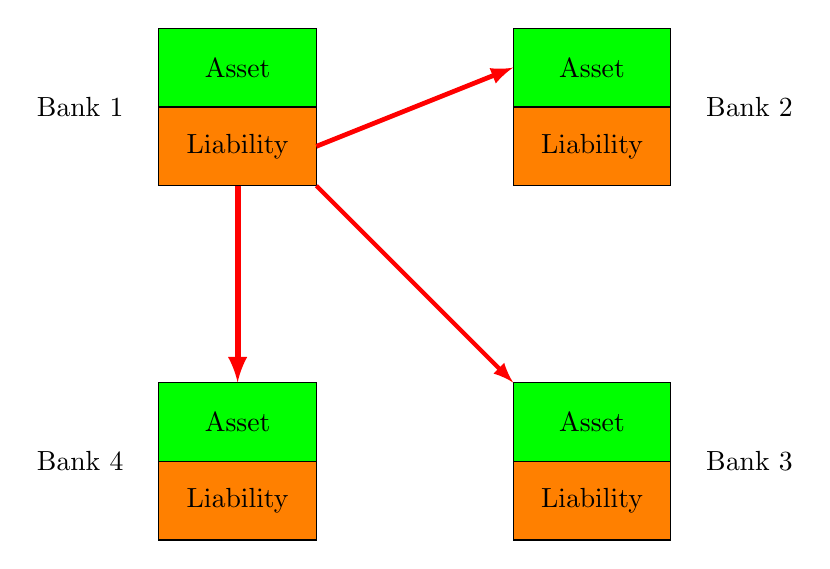
\begin{tikzpicture}
	    % First column
		\draw[fill=orange] (0,0) rectangle (4/2,2/2) node[pos=.5]{Liability};
		\draw[fill=green](0,2/2) rectangle (4/2,4/2) node[pos=.5]{Asset};
		\draw[fill=orange] (0,9/2) rectangle (4/2,11/2) node[pos=.5]{Liability};
		\draw[fill=green](0,11/2) rectangle (4/2,13/2)node[pos=.5]{Asset};		
		% Second column
		\draw[fill=orange] (9/2,0) rectangle (13/2,2/2) node[pos=.5]{Liability};
		\draw[fill=green](9/2,2/2) rectangle (13/2,4/2)node[pos=.5]{Asset};
		\draw[fill=orange] (9/2,9/2) rectangle (13/2,11/2) node[pos=.5]{Liability};
		\draw[fill=green](9/2,11/2) rectangle (13/2,13/2)node[pos=.5]{Asset};		
		% Name banks
		\node at (-2/2,11/2) {Bank 1};
		\node at (15/2,11/2) {Bank 2};
		\node at (-2/2, 2/2) {Bank 4};
		\node at (15/2, 2/2) {Bank 3};
		% Draw arrows
		\draw[-latex,red,line width=.5ex] (2/2,9/2) -- (2/2,4/2);
		\draw[-latex,red,line width=.4ex] (4/2,10/2) -- (9/2,12/2);
		\draw[-latex,red,line width=.35ex] (4/2,9/2) -- (9/2,4/2);
	\end{tikzpicture}
\end{center}
\tiny{Source: Chan-Lau (2013)}
\end{frame}

\begin{frame} % Example 4: Every firm is systemic
\frametitle{Example 4: Every firm is systemic}
\begin{center}
	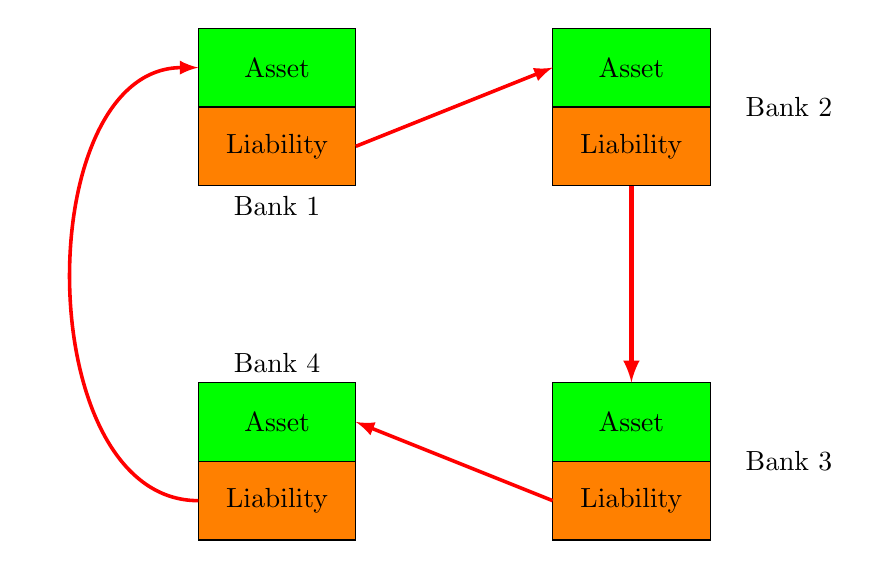
\begin{tikzpicture}
	    % First column
		\draw[fill=orange] (0,0) rectangle (4/2,2/2) node[pos=.5]{Liability};
		\draw[fill=green](0,2/2) rectangle (4/2,4/2) node[pos=.5]{Asset};
		\draw[fill=orange] (0,9/2) rectangle (4/2,11/2) node[pos=.5]{Liability};
		\draw[fill=green](0,11/2) rectangle (4/2,13/2)node[pos=.5]{Asset};		
		% Second column
		\draw[fill=orange] (9/2,0) rectangle (13/2,2/2) node[pos=.5]{Liability};
		\draw[fill=green](9/2,2/2) rectangle (13/2,4/2)node[pos=.5]{Asset};
		\draw[fill=orange] (9/2,9/2) rectangle (13/2,11/2) node[pos=.5]{Liability};
		\draw[fill=green](9/2,11/2) rectangle (13/2,13/2)node[pos=.5]{Asset};		
		% Name banks
		\node at (2/2,8.5/2) {Bank 1};
		\node at (15/2,11/2) {Bank 2};
		\node at (2/2, 4.5/2) {Bank 4};
		\node at (15/2, 2/2) {Bank 3};
		% Draw arrows
		\draw[-latex,red,line width=0.3ex] (4/2,10/2) -- (9/2,12/2);
		\draw[-latex,red,line width=0.4ex] (11/2,9/2) -- (11/2,4/2);
		\draw[-latex,red,line width=0.3ex] (9/2,1/2) -- (4/2,3/2);
		\draw[-latex,red,line width=0.3ex] (0/2,1/2) to[bend left=90](0/2,12/2);
	\end{tikzpicture}
\end{center}
\tiny{Source: Chan-Lau (2013)}
\end{frame}

\subsection{Centrality measures}

\begin{frame} % Why Topology Matters
\begin{center}
	\Large{Centrality measures}
\end{center}
\end{frame}

\begin{frame} % Centrality Measures
\frametitle{Centrality measures (1)}
Apply to any type of network
\vspace{1cm}
\begin{itemize}
	\item Strength
	\smallskip
	\item Closeness
	\smallskip
	\item Eigenvector centrality
	\smallskip
	\item PageRank
\end{itemize}
\end{frame}

\begin{frame} % Centrality Measures
\frametitle{Centrality measures (2)}
\begin{center}
	\includegraphics[scale=0.35]{figures/figWellsFargo.eps}
\end{center}
\end{frame}

\subsection{Counterfactual default simulation}

\begin{frame} % Counterfactual default simulations
\begin{center}
	\Large{Counterfactual default simulations}
\end{center}
\end{frame}

\begin{frame} % Default cascade algorithm
\frametitle{Default cascade algorithm}
Follows groundwork set by Eisenberg and Noe (2001)
\vspace{0.5mm}
\begin{enumerate}
\setbeamertemplate{enumerate items}[default]
	\item Construct matrix of interfirm exposure
	\smallskip
	\item Firm $i$ fails by assumption
	\smallskip
	\item Any firm $j$ fails
		\begin{itemize}
			\item Losses exceed capital
			\item Capital falls below threshold
		\end{itemize}
	\smallskip
	\item Second round of contagion prompted by failure of $j$ firms
\end{enumerate}
\vspace{1ex}
\color{red}{Don't forget: it is just a snapshot at time data was collected!}
\end{frame}

\begin{frame} % Default cascade
\frametitle{Default cascade}
\begin{center}
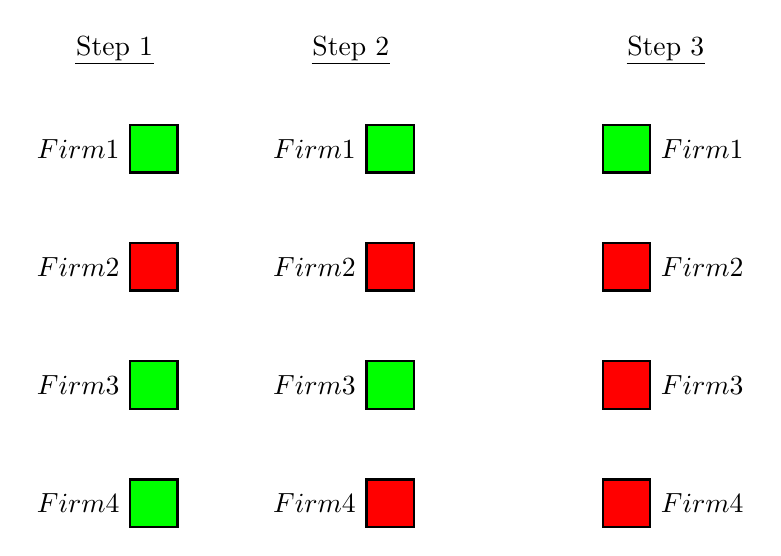
\begin{tikzpicture}
	[firm/.style={circle,draw=blue, fill=blue!70, thick,
				   inner sep=0pt, minimum size=6mm},
	 risk/.style={rectangle, inner sep=0pt, minimum size=6mm}]
%	\draw[draw=black, fill=orange!50] (-2,-0.5) rectangle ++(3,6.25);
%	\draw[draw=black, fill=green!30] (2,-0.5) rectangle ++(3,6.25);

	\node at (-3.5,5.75){\uline{Step 1}};
	\node at (-0.5,5.75){\uline{Step 2}};	
	\node at (3.5,5.75) {\uline{Step 3}};	 
	
	\node at (-3,0)    [risk,draw=black, fill=green, thick](rf4)
					  [label=left:$\text{Firm }4$]{};
	\node at (-3,1.5)  [risk,draw=black, fill=green,thick](rf3)
	                  [label=left:$\text{Firm }3$]{};
	\node at (-3,3.0)  [risk,draw=black, fill=red, thick](rf2)
				   	  [label=left:$\text{Firm }2$]{};
	\node at (-3,4.5)  [risk,draw=black, fill=green, thick](rf1)
	                  [label=left:$\text{Firm }1$]{};
	                  
	\node at (0,0)    [risk,draw=black, fill=red, thick](rf4)
					  [label=left:$\text{Firm }4$]{};
	\node at (0,1.5)  [risk,draw=black, fill=green,thick](rf3)
	                  [label=left:$\text{Firm }3$]{};
	\node at (0,3.0)  [risk,draw=black, fill=red, thick](rf2)
				   	  [label=left:$\text{Firm }2$]{};
	\node at (0,4.5)  [risk,draw=black, fill=green, thick](rf1)
	                  [label=left:$\text{Firm }1$]{};
	                  	                  
	\node at (3,0)    [risk,draw=black, fill=red, thick](rf4)
					  [label=right:$\text{Firm }4$]{};
	\node at (3,1.5)  [risk,draw=black, fill=red,thick](rf3)
	                  [label=right:$\text{Firm }3$]{};
%    \node[red, below] at (3.5,1.25){$PD_j(1+\delta)$};
	\node at (3,3.0)  [risk,draw=black, fill=red, thick](rf2)
				   	  [label=right:$\text{Firm }2$]{};
	\node at (3,4.5)  [risk,draw=black, fill=green, thick](rf1)
	                  [label=right:$\text{Firm }1$]{};
\end{tikzpicture}
\end{center}
\end{frame}


\begin{frame} % Credit shock
\frametitle{Credit shock}
\begin{center}
	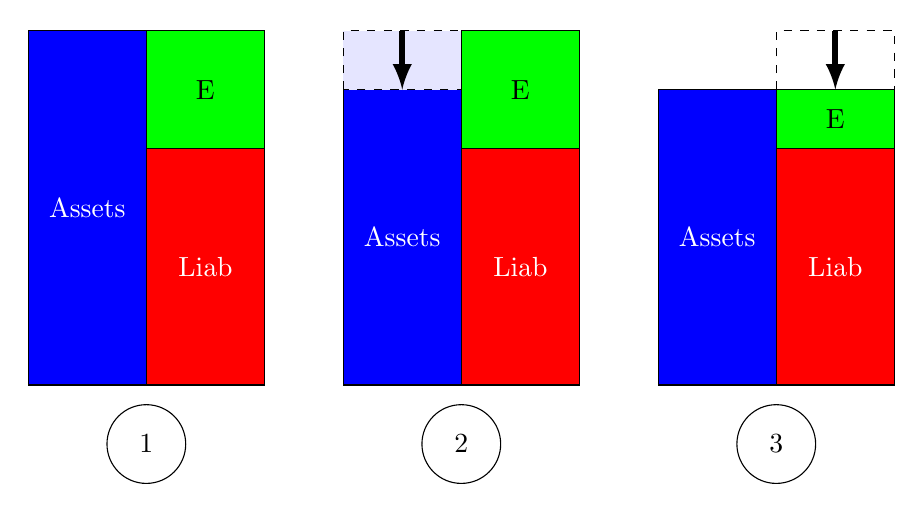
\begin{tikzpicture}
		% first step
		\draw[fill=blue](0,0) rectangle (3/2,9/2) node[white,pos=.5]{Assets};
		\draw[fill=red] (3/2,0) rectangle (6/2,6/2)  node[white,pos=.5]{Liab};
		\draw[fill=green](3/2,6/2) rectangle (6/2,9/2) node[pos=.5]{E};
		\draw (3/2,-3/4) circle [radius=5mm] node {1};
	    % second step
		\draw[fill=blue](0+4,0) rectangle (3/2+4,7.5/2) node[white,pos=.5]{Assets};		
		\draw[fill=red] (3/2+4,0) rectangle (6/2+4,6/2)  node[white,pos=.5]{Liab};
		\draw[fill=green](3/2+4,6/2) rectangle (6/2+4,9/2) node[pos=.5]{E};
		\draw[dashed, fill=blue!10] (0+4,7.5/2) rectangle (3/2+4,9/2);
		\draw[-latex,black,line width=0.5ex] (0+4+1.5/2,9/2) -- (0+4+1.5/2,7.5/2);
		\draw (3/2+4,-3/4) circle [radius=5mm] node {2};
        % third step
		\draw[fill=blue](0+8,0) rectangle (3/2+8,7.5/2) node[white,pos=.5]{Assets};		
		\draw[fill=red] (3/2+8,0) rectangle (6/2+8,6/2)  node[white,pos=.5]{Liab};
		\draw[fill=green](3/2+8,6/2) rectangle (6/2+8,7.5/2) node[pos=.5]{E};
		\draw[dashed] (3/2+8,7.5/2) rectangle (6/2+8,9/2);
		\draw[-latex,black,line width=0.5ex] (3/2+8+1.5/2,9/2) -- (3/2+8+1.5/2,7.5/2);
		\draw (3/2+8,-3/4) circle [radius=5mm] node {3};	
	\end{tikzpicture}
\end{center}
\end{frame}

\begin{frame} % Funding shock
\frametitle{Funding shock}
\begin{center}
	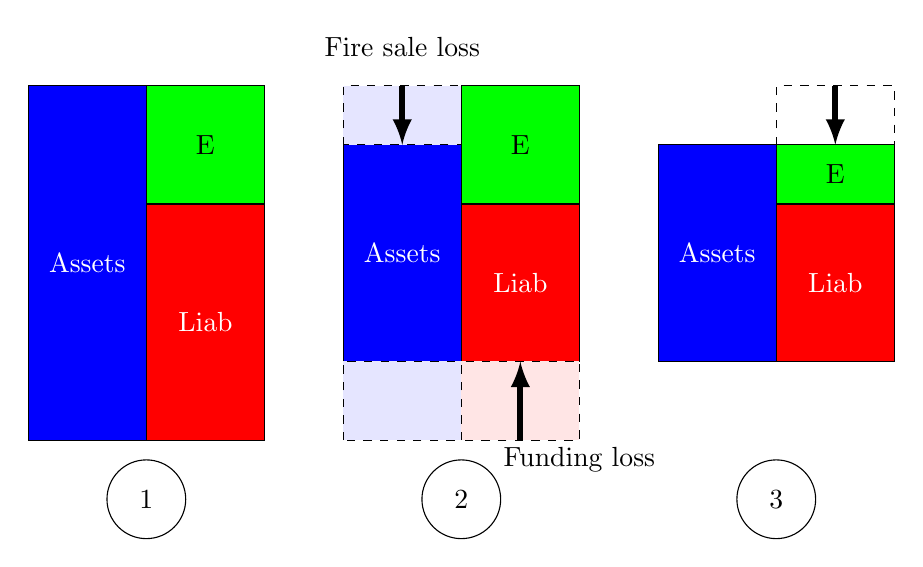
\begin{tikzpicture}
		% first step
		\draw[fill=blue](0,0) rectangle (3/2,9/2) node[white,pos=.5]{Assets};
		\draw[fill=red] (3/2,0) rectangle (6/2,6/2)  node[white,pos=.5]{Liab};
		\draw[fill=green](3/2,6/2) rectangle (6/2,9/2) node[pos=.5]{E};
		\draw (3/2,-3/4) circle [radius=5mm] node {1};
	    % second step
		\draw[fill=blue](0+4,2/2) rectangle (3/2+4,7.5/2) node[white,pos=.5]{Assets};		
		\draw[dashed,fill=blue!10] (0+4,0) rectangle (3/2+4,2/2); 
		\draw[fill=red] (3/2+4,2/2) rectangle (6/2+4,6/2)  node[white,pos=.5]{Liab};
		\draw[fill=green](3/2+4,6/2) rectangle (6/2+4,9/2) node[pos=.5]{E};
		\draw[dashed,fill=blue!10] (0+4,7.5/2) rectangle (3/2+4,9/2);
		\draw[dashed,fill=red!10] (3/2+4,0) rectangle (6/2+4,2/2);
		\draw[-latex,black,line width=0.5ex] (0+4+1.5/2,9/2) -- (0+4+1.5/2,7.5/2);
		\draw[-latex,black,line width=0.5ex] (3/2+4+3/4,0) -- (3/2+4 +3/4,2/2);		
		\node at (3/4+4,9/2 + 1/2) {Fire sale loss};
		\node at (6/2+4,-1/4) {Funding loss};
		\draw (3/2+4,-3/4) circle [radius=5mm] node {2};
        % third step
		\draw[fill=blue](0+8,2/2) rectangle (3/2+8,7.5/2) node[white,pos=.5]{Assets};		
		\draw[fill=red] (3/2+8,2/2) rectangle (6/2+8,6/2)  node[white,pos=.5]{Liab};
		\draw[fill=green](3/2+8,6/2) rectangle (6/2+8,7.5/2) node[pos=.5]{E};
		\draw[dashed] (3/2+8,7.5/2) rectangle (6/2+8,9/2);
		\draw[-latex,black,line width=0.5ex] (3/2+8+1.5/2,9/2) -- (3/2+8+1.5/2,7.5/2);
		\draw (3/2+8,-3/4) circle [radius=5mm] node {3};	
	\end{tikzpicture}
\end{center}
\end{frame}

\begin{frame} % Workshop Excel Worksheet
	\Large{Hands-On Exercise 1:\\
	Network analysis in Excel}\\
	\vspace{1em}
	\Large{Espinosa and Sole (2010)}
\end{frame}

\subsection{Modeling additional second-round effects}

\begin{frame} % Modeling additional second-round effects
\begin{center}
	\Large{Modeling additional second round-effects}
\end{center}
\end{frame}

\begin{frame} % Additional second-round effects (1)
\frametitle{Additional second-round effects (1)}
\begin{itemize}
	\item Counterfactual simulations
	\begin{itemize}
		\item Require failure of a firm
		\item Shocks work only through inter-firm exposures
		\item Nothing happens if no firm defaults
	\end{itemize}
	\smallskip
\end{itemize}
\end{frame}

\begin{frame} % Additional second-round effects (2)
\frametitle{Additional second round effects (2)}
\textbf{Funding cost model (Jo, 2012)}
\begin{itemize}
	\item Capital ratios reflect risk of firm
	\item Higher risk $\Rightarrow$ lower funding replacement rate
	\item Higher risk $\Rightarrow$ higher funding costs
\end{itemize}
\begin{center}
	\includegraphics[scale=0.3]{figures/figJo2012.eps}
\end{center}
\tiny{Source: Jo (2012)}
\end{frame}

\begin{frame} % Additional second-round effects (3)
\frametitle{Additional second round effects (3)}
\begin{center}
	\includegraphics[scale=0.33]{figures/figJoSimulation.eps}
\end{center}
\tiny{Source: Sun and Chan-Lau (2017)}
\end{frame}

\begin{frame} % Additional second-round effects (4)
\frametitle{Additional second round effects (4)}
\textbf{DebtRank (Bardoscia et al, 2015)}
\vspace{4mm}
\begin{itemize}
	\item Second-round effects from counterparty risk
	\smallskip
	\item Inter-firm exposure reflects changing default risk
	\smallskip
	\item Analogous to counterparty valuation adjustment (CVA)
	\smallskip
	\item The trick
	\begin{itemize}
		\item Value of claim on firm depends on firms' change in equity value
		\item Equity value falls $\Rightarrow$ value on claim falls
	\end{itemize}
	\smallskip
	\item Default is no longer necessary for contagion
\end{itemize}
\end{frame}

\begin{frame} % Additional second-round effects (5)
\frametitle{Additional second round effects (5)}
\begin{center}
\scriptsize{Impact and vulnerability of European banks in 2008, 0.5 percent asset price decline}
	\includegraphics[scale=0.35]{figures/figDebtRankScatter.eps}
\end{center}
\tiny{Source: Bardoscia et al (2015)}
\end{frame}

\subsection{Some caveats with direct exposures networks}

\begin{frame}
\begin{center}
	\Large{Caveats}
\end{center}
\end{frame}

\begin{frame} % Caveats when using BIS banking data
\frametitle{Caveats when using BIS banking data (1)}
\begin{center}
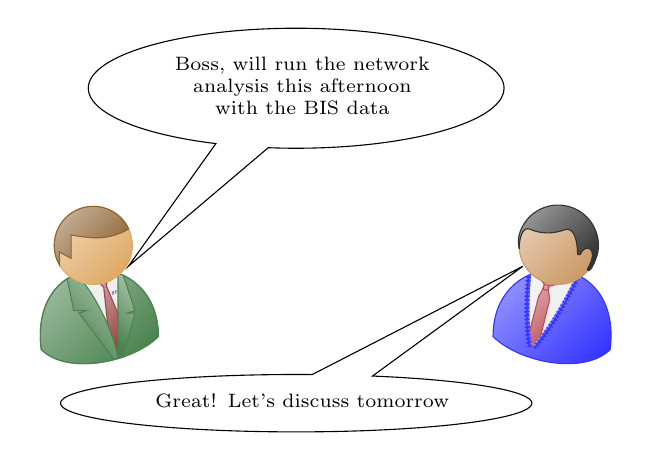
\begin{tikzpicture}
%	\node[businessman,evil, female, minimum size = 1.5cm] at (0,0){};
	\node[name=a,shape=businessman, minimum size=1.5cm,xshift=-2.50cm] {};
	\node[dave, shirt=blue,skin=brown, name=b,minimum size=1.5cm,mirrored,xshift=3.25cm] {};
	\node[draw, ellipse callout, yshift= 2.5cm, callout absolute pointer={(a.mouth)},
	font=\scriptsize, text width=3.5cm] {\begin{tabular}{c} Boss, will run the network\\ analysis this afternoon\\ with the BIS data \end{tabular}};
	\node[draw, ellipse callout, yshift= -1.5cm, callout absolute pointer={(b.mouth)},
	font=\scriptsize, text width=4cm] {\begin{tabular}{c} Great! Let's discuss tomorrow \end{tabular}};
\end{tikzpicture}
\end{center}
\end{frame}

\begin{frame} % Caveats when using BIS banking data
\frametitle{Caveats when using BIS banking data (2)}
\begin{center}
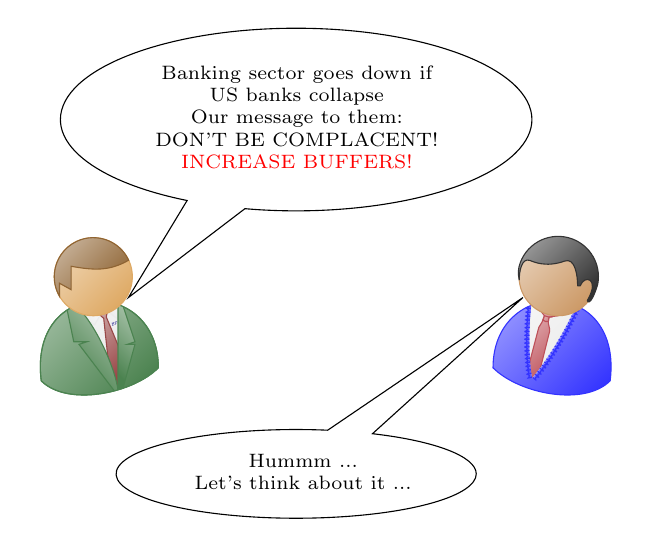
\begin{tikzpicture}
%	\node[businessman,evil, female, minimum size = 1.5cm] at (0,0){};
	\node[name=a,shape=businessman, minimum size=1.5cm,xshift=-2.50cm] {};
	\node[dave, shirt=blue,skin=brown, name=b,minimum size=1.5cm,mirrored,xshift=3.25cm] {};
	\node[draw, ellipse callout, yshift= 2.5cm, callout absolute pointer={(a.mouth)},
	font=\scriptsize, text width=4cm] {\begin{tabular}{c} Banking sector goes down if \\US banks collapse\\ 
	Our message to them: \\DON'T BE COMPLACENT!\\ \color{red}{INCREASE BUFFERS!} \end{tabular}};
	\node[draw, ellipse callout, yshift= -2.0cm, callout absolute pointer={(b.mouth)},
	font=\scriptsize, text width=3cm] {\begin{tabular}{c} Hummm ... \\Let's think about it ... \end{tabular}};
\end{tikzpicture}
\end{center}
\end{frame}

\begin{frame} % Multiplex networks (1)
\frametitle{Multiplex (multi-layer) networks (1) }
\begin{center}
	\includegraphics[scale=0.40]{figures/figSunChanLauTable.eps}
\end{center}
\tiny{Source: Sun and Chan-Lau (2017)}
\end{frame}

\begin{frame} % Multiplex networks (1)
\frametitle{Multiplex (multi-layer) networks (2) }
\begin{center}
	\includegraphics[scale=0.38]{figures/figdataLosses.eps}
\end{center}
\tiny{Source: Chan-Lau (2010)}
\end{frame}

\section{Market-based networks}

\subsection{Correlation Approaches}

\begin{frame} % Correlation Approaches
\begin{center}
	\Large{Correlation approaches}
\end{center}
\end{frame}

\begin{frame} % Correlation approaches (1)
\frametitle{Correlation approaches (1)}
\begin{itemize}
	\item Basic idea
		\begin{itemize}
			\item Time series of market prices, i.e. CDS, PDs, equity returns
			\item Find correlation-type matrix
			\item Matrix defines network
		\end{itemize}
	\smallskip
	\item Systemic risk assessment
		\begin{itemize}
			\item Centrality measures
		\end{itemize}
	\smallskip
	\item Some issues
		\begin{itemize}
			\item Plain correlation creates undirected edges
			\item Unstable correlation matrix 
			\item Correlation-based measures may capture third-party effects
		\end{itemize}
\end{itemize}
\end{frame}

\begin{frame} % Correlation approaches (2)
\frametitle{Correlation approaches (2)}
\begin{itemize}
	\item Some solutions
		\begin{itemize}
			\item Granger-causality networks
			\item Partial correlation networks
			\item Regularized correlation networks
		\end{itemize}
	\smallskip
	\item Solutions do not apply to multi-layer networks!
		\begin{itemize}
			\item Ad-hoc methods needed
		\end{itemize}
\end{itemize}
\end{frame}

\begin{frame} % Grange-causality network 
\frametitle{Granger-Causality network}
\begin{center}
	\includegraphics[scale=0.45]{figures/figGrangerCausality.eps}
\end{center}
\tiny{Source: Billio et al (2012)}
\end{frame}

\begin{frame} % Partial correlation network (1)
\frametitle{Partial correlation network (1)}
\begin{itemize}
	\item Granger causality networks are very dense
	\smallskip
	\item Trim or remove some of the edges
	\smallskip
	\item Potential solution: minimum spanning tree
	\smallskip
	\item But may remove too many edges
\end{itemize}
\begin{center}
\includegraphics[scale=0.55]{figures/figMST.eps}
\end{center}
\end{frame}

\begin{frame} % Partial correlation network(2)
\frametitle{Partial correlation network (2)}
\begin{itemize}
	\item Firms A, B, and C
	\smallskip
	\item Correlation between A and B due to
		\begin{itemize}
			\item Correlation between A and C
			\item Correlation between B and C
		\end{itemize}
	\smallskip
	\item Partial correlation removes effect of C
\end{itemize}
\end{frame}

\begin{frame} % Partial correlation network(3)
\frametitle{Partial correlation network (3)}
\begin{center}
	\includegraphics[scale=0.25]{figures/figPartialCorrelation.eps}
\end{center}
\tiny{Source: Kenett et al (2010)}
\end{frame}

\begin{frame} % Regularized partial correlation networks (1)
\frametitle{Regularized partial correlation network (1)}
\begin{itemize}
	\item Partial correlation may leave some firms orphan
	\smallskip
	\item There should be no orphans in a fully connected network
	\smallskip
	\item Arguably, financial networks should be fully connected
	\smallskip
	\item Use regularization trick
	\begin{itemize}
		\item Add penalty to trim procedure
		\item Remove edges gradually
		\item Stop just before first orphan emerges
	\end{itemize}
\end{itemize}
\end{frame}

\begin{frame} % Regularized partial correlation networks (2)
\frametitle{Regularized partial correlation network (2)}
\begin{center}
	\includegraphics[scale=0.3]{figures/figDefaultCorrelation.eps}
\end{center}
\tiny{Source: Chan-Lau, Chuang, Duan, and Sun (2017)\\
Monthly updates for 1928 firms at \color{red}{\textbf{\url{https://rmicri.org/en/srt/}}}}
\end{frame}

\begin{frame} % Regularized partial correlation networks (3)
\frametitle{Regularized partial correlation network (3)}
\begin{center}
	\includegraphics[scale=0.55]{figures/figDefaultCorrelationGFSR.eps}
\end{center}
\tiny{Source: IMF. 2016. Global Financial Stability Report, April}
\end{frame}

\subsection{Quantile regression approaches}

\begin{frame} % Quantile Regression cover page
\begin{center}
	\Large{Quantile regression approaches}
\end{center}
\end{frame}

\begin{frame} % Quantile regression (1)
\frametitle{Quantile regression (1)}
	\begin{itemize}
		\item Richer representation of data beyond mean response
		\smallskip
		\item Whole distribution of responses to covariates
		\smallskip
		\item Semiparametric approach requires no error distribution assumption
		\smallskip
		\item Uses all data points
		\smallskip
		\item Robust to non-normal errors and outliers
		\smallskip
		\item Invariant to transformation
	\end{itemize}
\end{frame}

\begin{frame} % Quantile regression (2)
\frametitle{Quantile Regression (2)}
\begin{center}
	\includegraphics[scale=0.5]{figures/figMexicoNPL.eps}
\end{center}
\end{frame}

\begin{frame} % Quantile regression (3)
\frametitle{Quantile Regression (3)}
\begin{center}
The crossing line problem \end{center}
\begin{center}
	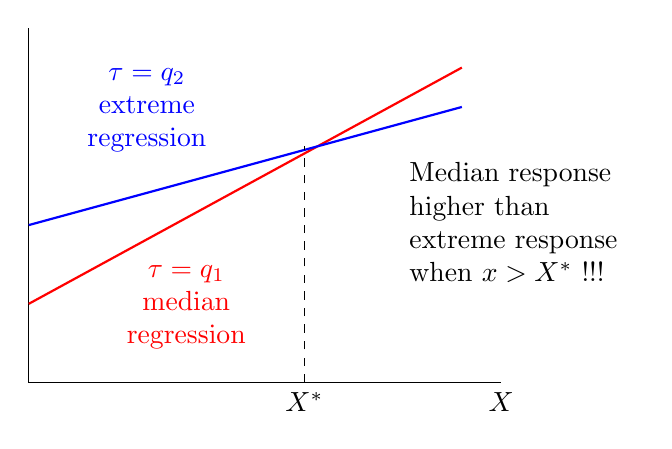
\begin{tikzpicture}
		\draw (0,0) -- (6,0);
		\draw (0,0) -- (0,4.5);
%		\draw[step=0.5cm, thin] (0,0) grid (5.5, 4.5);		
		\draw[red, thick] (0,1) -- +(5.5,3);
		\draw[blue,thick] (0,2) -- +(5.5,1.5);
		\draw[dashed] (3.5,0) -- (3.5,3);
		\node[red] at (2.0,1.0){\begin{tabular}{c} 
			$\tau = q_1$\\
			median\\
			regression
			\end{tabular}};
		\node[blue] at (1.5,3.5){\begin{tabular}{c}
			$\tau = q_2$\\
			extreme\\
			regression
			\end{tabular}};
		\node[below] at (3.5,0){$X^*$};
		\node[below] at (6,0){$X$};
		\node[right] at (4.5,2){\begin{tabular}{l} Median response\\
		higher than\\ 
		extreme response\\
		when $x > X^*$ !!! 
		\end{tabular}};
	\end{tikzpicture}
\end{center}
\end{frame}

\begin{frame} % Quantile regression (4)
\frametitle{Quantile Regression (4)}
\begin{center}
\scriptsize{
Extreme QR yields "less extreme" outcome than median QR}
\end{center}
\begin{center}
	\begin{tikzpicture}
		\draw (0,0) -- (6,0);
		\draw (0,0) -- (0,4.5);
%		\draw[step=0.5cm, thin] (0,0) grid (5.5, 4.5);		
		\draw[red, thick] (0,1) -- +(5.5,3);
		\draw[blue,thick] (0,2) -- +(5.5,1.5);
		\draw[dashed, thick] (4.5,0) -- (4.5,3.5);
%		\node[below] at (3.5,0){$X^*$};
		\node[below] at (6,0){$X$};
		\node[below] at (4.5,0){\color{teal}{$X_{99}$}};		
	\end{tikzpicture}
\end{center}
\end{frame}

\begin{frame} % Quantile regression (5)
\frametitle{Quantile Regression (5)}
\begin{center}
\scriptsize{Good riddance to median QR; introduce $X_{50}$;\\
systemic risk is $QR_{xtr}(X_{99}) - QR_{xtr}(X_{50})$}
\end{center}
\begin{center}
	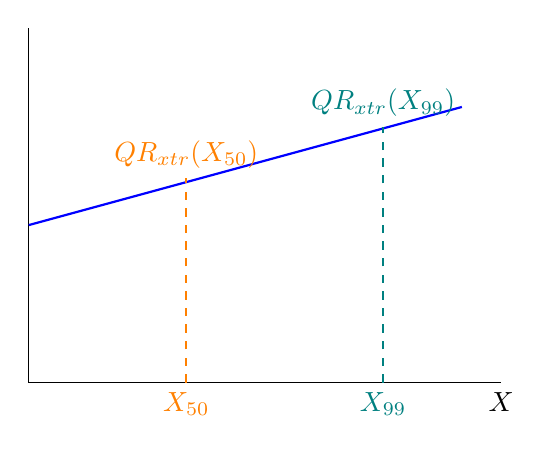
\begin{tikzpicture}
		\draw (0,0) -- (6,0);
		\draw (0,0) -- (0,4.5);
%		\draw[step=0.5cm, thin] (0,0) grid (5.5, 4.5);		
%		\draw[red, thin, dashed] (0,1) -- +(5.5,3);
		\draw[blue,thick] (0,2) -- +(5.5,1.5);
		\draw[dashed,teal,thick] (4.5,0) -- (4.5,3.25);
%		\node[below] at (3.5,0){$X^*$};
		\node[below] at (6,0){$X$};
		\node[below] at (4.5,0){\color{teal}{$X_{99}$}};		
		\node[below] at (2,0){\color{orange}{$X_{50}$}};				
		\draw[dashed,thick, orange] (2,0) -- (2,2.6);
		\node[above, orange] at (2,2.6){$QR_{xtr}(X_{50})$};
		\node[above, teal] at (4.5,3.25){$QR_{xtr}(X_{99})$};
	\end{tikzpicture}
\end{center}
\end{frame}

\begin{frame} % CoVaR Cover page
\begin{center} 
	\Large{Quantile regression approaches:\\CoVaR}
\end{center}
\end{frame}

\begin{frame} % CoVaR (1)
\frametitle{CoVaR (1)}
\begin{itemize}
	\item Adrian and Brunnermeier (2016)
	\smallskip
	\item $X_i$ risk measure of firm $i$
	\smallskip
	\item Lower $X_i$, higher risk
	\smallskip
	\item Value-at-Risk, $q-th$ quantile
	\begin{equation*}
		\Pr \left(X_i \leq VaR_{q}^i \right) = q
	\end{equation*}
	\item Unconditional tail risk, $q$ small, i.e. 1\%
\end{itemize}
\end{frame}

\begin{frame} % CoVaR (2)
\frametitle{CoVaR (2)}
\begin{center}
	\includegraphics[scale=0.2]{figures/figCoVaR1.eps}
\end{center}
\tiny{Source: Chan-Lau, J.A. 2017. \textit{Quantile regressions and extreme value theory in financial regulation}\\Lecture Notes, SBS Workshop, Lima, Per\'u}
\end{frame}

\begin{frame} % CoVaR (3)
\frametitle{CoVaR (3)}
\begin{itemize}
	\item Systemic risk focused on {\color{red}{contagion}}
	\smallskip
	\item Contagion = distress of $A$ conditional on distress of $B$
	\smallskip
	\item $C(B)$ event affecting $B$
	\smallskip
	\item $CoVaR_{q}^{A|C(B)}$ satisfies
	\begin{equation*}
		\Pr \left([ X_A|C(B) \leq CoVaR_{q}^{A|C(B)}] \right) = q	
	\end{equation*}
\end{itemize}
\end{frame}

\begin{frame} % CoVaR (4)
\frametitle{CoVaR (4)}
\begin{center}
\scriptsize{Event $C(B)$ affects location and scale of original P/L distribution}
\end{center}
\begin{center}
	\includegraphics[scale=0.2]{figures/figCoVaR2.eps}
\end{center}
\tiny{Source: Chan-Lau, J.A. 2017. \textit{Quantile regressions and extreme value theory in financial regulation}\\Lecture Notes, SBS Workshop, Lima, Per\'u}
\end{frame}

\begin{frame} % Delta CoVaR (1)
\frametitle{$\Delta CoVaR$ (1)}
\begin{itemize}
	\item Event $C(B)$ can be \textbf{{\color{blue}{normal}}} or \textbf{{\color{red}{extreme}}}
	\smallskip
	\item {\colorbox{blue}{\color{white}{{Normal event}}}}
	\begin{equation*}
		\left\{X_B = VaR_{q_{normal}}^B, {\color{blue}{q_\text{extreme} = 0.5}} \right\}
	\end{equation*}
	\item {\colorbox{red}{\color{white}{Extreme event}}}
	\begin{equation*}
		\left\{X_B = VaR_{q_{extreme}}^B, {\color{red}{q_\text{extreme} = 0.01}} \right\}
	\end{equation*}
	\smallskip
	\begin{center}
	\boxed{
		\Delta CoVaR_{q}^{A|B} = CoVaR_{q}^{A|VaR_{q}^B} - CoVaR_{q}^{A|VaR_{0.5}^B}
	}	
	\end{center}
\end{itemize}
\end{frame}

\begin{frame} % Delta CoVaR (2)
\frametitle{$\Delta CoVaR$ (2)}
\begin{itemize}
	\item Extreme quantile regression estimation
	\begin{equation*}
		X_A = \alpha(\tau) + \beta(\tau) X_B, \tau = q; \hspace{2em}  q={\color{red} q_\text{extreme}}
	\end{equation*}
	\item $CoVaR$ estimation
	\begin{equation*}
		CoVaR_q^{A|\textit{VaR}_q^B} = \alpha(\tau=q) + \beta(\tau=q)\textit{VaR}_q^B
	\end{equation*}
	\begin{equation*}
		CoVaR_{q}^{A|\textit{VaR}_{50}^B} = \alpha(\tau=q) + \beta(\tau=q)\textit{VaR}_{0.5}^B
	\end{equation*}
	\item $\Delta CoVaR$ estimation
	\begin{equation*}
		\Delta CoVaR_{q}^{A|B} = \beta(\tau=q) \times \left( VaR_{q}^B - VaR_{0.5}^B \right)
	\end{equation*}
\end{itemize}
\end{frame}

\begin{frame} % Delta CoVaR (3)
\frametitle{$\Delta CoVaR$ (3)}
\begin{center}
	\includegraphics[scale=0.35]{figures/figCoVaR.eps}
\end{center}
\tiny{IMF, GFSR April 2016}
\end{frame}

\begin{frame} % Hands-on workshop: CoVaR
	\Large{Hands-on-Exercise 2:\\
	$\Delta CoVaR$ }\\
	\vspace{1em}
	\Large{Adrian and Brunnermeier (2016)}
	
\href{https://htmlpreview.github.io/?https://github.com/jchanlauimf/Systemic-Risk/blob/master/CoVaR/CoVaR_Tutorial.html}{\beamergotobutton{Tutorial page}}		
\end{frame}

\begin{frame} % CoRisk cover page
\begin{center} 
	\Large{Quantile regression approaches:\\CoRisk}
\end{center}
\end{frame}

\begin{frame} % CoRisk (1)
\frametitle{CoRisk (1)}
	\begin{itemize}
		\item Pick any relevant risk measure, i.e. $PD$
		\smallskip
		\item Pick an upper quantile $\tau$, i.e. $\tau = 0.95$
		\smallskip
		\item Quantile regression of $i$ on $j$ and risk factors $X$
		\begin{equation*}
			PD_i = QR(PD_j,X_k; \tau) =  \alpha_{\tau} + \beta_{\tau} PD_j + \sum_k \beta_{\tau,k} X_k
		\end{equation*}
		\item Find the unconditional $\tau$ and median ($q=0.50$) quantiles for $PD_i$, $PD_j$
	\end{itemize}
\end{frame}

\begin{frame} % CoRisk (2)
\frametitle{CoRisk (2)}
	\begin{itemize}
		\item CoRisk (in levels)
		\begin{equation*}
		\begin{split}
		\text{CoRisk} &= QR(PD_j(\tau), X_k(q); \tau) - QR(PD_j(q), X_k(q); \tau)\\	
		&= \beta_{\tau} \left( PD_j(\tau) - PD_j(q) \right)
		\end{split}	
		\end{equation*}
		\item CoRisk (in percent)
		\begin{equation*}
		\text{CoRisk} = \frac{\beta_{\tau} \left( PD_j(\tau) - PD_j(q) \right)}
			{PD_i(q)}
		\end{equation*}
	\end{itemize}	
\end{frame}

\subsection{Variance decomposition approaches}

\begin{frame} % Diebold Yilmaz cover page
\begin{center}
	\Large{Variance decomposition approaches:\\
	Diebold-Yilmaz}
\end{center}
\end{frame}

\begin{frame} % Diebold Yilmaz basics (1)
  \frametitle{Diebold-Yilmaz (1): basics}
  \begin{itemize}
     \item Start selecting number of firms
     \smallskip
  	 \item Estimate unrestricted VAR model
  	 \begin{itemize}
  	 	\item Equity returns
  	 	\item Observable market-based measures
  	 \end{itemize}  	
  	 \smallskip
  	 \item Network construction
  	 \begin{itemize}
  	 	\item Each firm is a node
  	 	\item Edges
  	 	\begin{itemize}
  	 		\item Directional, i.e. from $i$ to $j$
  	 		\item Contribution of $i$ to variance decomposition of $j$
  	 	\end{itemize}
  	 \end{itemize}
  \end{itemize}
\end{frame}

\begin{frame} % Variance Decomposition (2)
  \frametitle{Diebold-Yilmaz (2): variance decomposition}
  \begin{itemize}
    \item Generalized Forecast Error Variance Decomposition (GFEVD)
    \begin{itemize}
      \item Introduced by Pesaran and Shin (1998)
      \item VAR ordering does not matter (Koop, Pesaran, and Potter, 1996)
    \end{itemize}
    \smallskip
    \item FEVD from structural VAR adds to unity ...
    \smallskip
    \item ... bug GFEVD does not!
    \begin{itemize}
    	\item Cross-effects of error terms
    \end{itemize}
  \end{itemize}
\end{frame}

\begin{frame} % Figure DY decomposition (3)
\frametitle{Diebold-Yilmaz (3): GFEVDs do not add to one}
  \begin{center}
    \includegraphics[height=2.75in]{figures/figDYcontributions.eps}  
  \end{center}
  \tiny{Source: Chan-Lau (2017)}
\end{frame}

\begin{frame} % Explain GFEVD (4)
\frametitle{Diebold-Yilmaz (4): patching up the GFEVD}
  \begin{itemize}
    \item Start with MA representation of VAR
    \[Y_t = \sum_{j=0}^{\infty} A_j \epsilon_{t-j} \]
    \item Pesaran-Shin GFEVD, horizon $h$
    \begin{equation*}
        \theta_{ij}(h) = \frac{\sigma_{ii}^{-1} \sum_{k=0}^{h}(e'_{j} A_k e_{j})^2}
    {\sum_{k=0}^{h} {e'_j} {A_k} \Sigma {A'_{k}} e_i}
    \end{equation*}     
    \item Diebold-Yilmaz normalization
    \smallskip
    \item[]
    \begin{center}
    \boxed{
%    \begin{equation*}
      \hat{\theta}_{ij}(h) = \frac{\theta_{ij}(h)}{\sum_{k=1}^{n} \theta_{ik}(h)}
%    \end{equation*}
	}    
    \end{center}
    \item Higher $\sum_{j=1,..,n}\hat{\theta}_{ij}$ implies higher systemic risk ranking 
  \end{itemize}
\end{frame}

\begin{frame} % GFSR Figure (5)
\frametitle{Diebold-Yilmaz (5): GFSR 2016, Chapter 3}
\begin{center}
	\includegraphics[scale=0.35]{figures/figGFSRDY.eps}
\end{center}
\end{frame}

\begin{frame} % GFSR Figure (5)
\frametitle{Diebold-Yilmaz (6): Germany Article IV, 2016}
\begin{center}
	\includegraphics[scale=0.65]{figures/figRiskDieboldYilmaz.png}
\end{center}
\begin{flushleft}
\tiny{Risk Magazine, online. November 2, 2017}
\end{flushleft}
\end{frame}

\begin{frame} % Problems with DY GFEVD (5)
\frametitle{Diebold-Yilmaz (7): pitfalls in interpreting DY GFEVD}
  \begin{itemize}
    \item Economic interpretation of shocks (Koop et al, 1996)
    \begin{itemize}
    	\item Cross-effects of error terms
    	\item GFEVD less, equal, or greater than one
    \end{itemize}
    \smallskip
    \item Ok for static analysis
    \begin{itemize}
    	\item Risk/vulnerability rankings at any point in time    	
    \end{itemize}
    \smallskip
    \item Inconsistent for assessing risk evolution over time   
  \end{itemize}
\vspace{.25cm}
\begin{flushleft}
	\tiny{*See also Kossner and Wagner (2014) on potential problems with Diebold-Yilmaz spillover indices}
\end{flushleft}  
\end{frame}

\begin{frame} % Pitfalls in a simple example (6)
\frametitle{Diebold-Yilmaz (8): simple pitfall example}
	\begin{itemize}
	  \item Period 1
	  	\begin{itemize}
	  		\item Firm A explains 20 percent of GFEVD of firm B
	  		\item Total GFEVD of firm B equals to 2
	  	\end{itemize}
	  \smallskip
	  \item Period 2
	  	\begin{itemize}
	  		\item Firm A explains 50 percent of GFEVD of firm B
	  		\item Total GFEVD of firm B equals to 0.5
	  	\end{itemize}	
	  \smallskip
	  \item Has Firm A become more systemic to Firm B?
	  \smallskip
	  \item Ambiguous answer
	  	\begin{itemize}
	  		\item Yes (DY normalization), up 50 percent from 20 percent
	  		\item No, 50 percent of 0.5 is less than 20 percent of 2
	  	\end{itemize}
	\end{itemize}
\end{frame}

\begin{frame} % Lanne Nyberg cover page
\begin{center} 
	\Large{Variance decomposition approaches:\\
	Lanne-Nyberg decompositions}
\end{center}
\end{frame}

\begin{frame} % Lanne-Nyberg (1)
\frametitle{Lanne-Nyberg (1): alternative decomposition}
\smallskip
	\begin{itemize}
		\item Diebold-Yilmaz network provide the right intuition but ...
		\smallskip
		\item ... variance decomposition method leads to ambiguous result
		\smallskip
		\item Ambiguity invalidates systemic risk ranking dynamics
		\smallskip
		\item How can we correct it?
		\smallskip
		\item \textbf{{\color{red}Use Lanne-Nyberg variance decomposition}}
	\end{itemize}
\end{frame}

\begin{frame} % Lanne Nyberg (2)
\frametitle{Lanne-Nyberg (2): Variance Decomposition}
	\begin{itemize}
		\item Starts with Generalized Impulse Response Function (GIRF)
		\begin{equation*}
			GI(h,\delta_t,\Omega_{t-1}) = A_h \Sigma e_j \sigma_{jj}^{-1} \delta_j	
		\end{equation*}
		\item Lanne-Nyberg GFEVD $\lambda_{ij}(h)$
		\smallskip
		\item[]
		\begin{center}
		\boxed{
%		\begin{equation*}
			\lambda_{ij}(h) = \frac{\sum_{k=0}^{h}GI(h,\delta_t,\Omega_{t-1})}
			{\sum_{j=1}^n \sum_{k=0}^{h}GI(h,\delta_t,\Omega_{t-1})}		
%		\end{equation*}
		}
		\end{center}
	\end{itemize}
\end{frame}

\begin{frame} % Case Study Diebold Yilmaz and Global Financial system (3)
\frametitle{Lanne-Nyberg(3): global financial system}
	\begin{itemize}
		\item Weekly equity returns 
			\begin{itemize}
				\item 402 firms
				\item 34 advanced and emerging market economies
			\end{itemize}
		\smallskip
		\item Sample dates
			\begin{itemize}
				\item Full sample: 01/01/2001 - 07/31/2016
				\item Pre-crisis period: 01/01/2001 - 12/31/2004
				\item Lehman Brothers: 01/01/2005 - 12/31/2008
				\item Sovereign debt crisis: 01/01/2009 - 12/31/2012
				\item Secular stagnation: 01/01/2013 - 07/31/2016
			\end{itemize}
		\smallskip
		\item Lasso Estimation, with 8 lags
		\smallskip
		\item Variance decomposition horizon = 52 weeks	
			\begin{itemize}
				\item Diebold-Yilmaz
				\item Lanne-Nyberg
			\end{itemize}
	\end{itemize}
\end{frame}

\begin{frame} % Divergences Lanne Nyberg Diebold Yilmaz (4)
\frametitle{Lanne-Nyberg (4): comparing systemic rankings}
	\begin{center}
		Number of overlapping firms in the top 50 DY and CLNDY rankings
		\includegraphics[height=2.5in]{figures/figOverlapping.eps}
	\end{center}
	\tiny{Source: Chan-Lau (2017)}
\end{frame}

\begin{frame} % FSAP Japan (5)
\frametitle{Lanne-Nyberg (5): FSAP Japan 2016 spillovers}
\begin{center}
	\includegraphics[scale=0.12]{figures/figTop2Japan.eps}
\end{center}
\end{frame}


\section{The portfolio approach}

\subsection{Credit loss distribution analogy}

\begin{frame} % Credit Loss Distribution Analogy Cover page
\begin{center} 
	\Large{Credit Loss Distribution Analogy}
\end{center}
\end{frame}

\begin{frame} % Credit Loss Distribution Analogy (1)
\frametitle{Credit loss distribution analogy (1)}
	\begin{itemize}
		\item Consider a set of firms
		\smallskip
		\item Group the firms in a credit portfolio
		\smallskip
		\item We will use loss distribution to assess a firm's systemic risk
		\smallskip
		\item Focus on tail risk measures
		\begin{itemize}
			\item Value-at-Risk (VaR)
			\item Expected Shortfall (ES)
		\end{itemize}
	\end{itemize}
\end{frame}

\begin{frame} % Credit Loss Distribution Analogy (2)
\frametitle{Credit loss distribution analogy (2)}
\begin{center}
	\includegraphics[scale=0.4]{figures/figCreditLoss.eps}
\end{center}
\end{frame}

\begin{frame} % Credit Loss Distribution Analogy (2)
\frametitle{Credit loss distribution analogy (3)}
	\begin{itemize}
		\item Increase default risk of a firm
		\begin{itemize}
			\item Loss distribution changes
			\item Tail risk measures change			
		\end{itemize}
		\smallskip
		\item Change in tail measure = systemic risk of firm
	\end{itemize}
\end{frame}

\subsection{Systemic risk contribution of a firm}

\begin{frame} % Systemic Risk distribution cover page
\begin{center} 
	\Large{Systemic risk contribution of a firm}
\end{center}
\end{frame}

\begin{frame} % Systemic risk contribution step 1
\frametitle{Systemic risk contribution of a firm (1)}
Step 1: Calculate loss distribution, firm under normal conditions
\begin{center}
	\includegraphics[scale=0.4]{figures/figSystemicContribution01.eps}
\end{center}
\end{frame}

\begin{frame} % Systemic risk contribution step 2
\frametitle{Systemic risk contribution of a firm (2)}
Step 2: Calculate the loss distribution when the firm is stressed
\begin{center}
	\includegraphics[scale=0.4]{figures/figSystemicContribution02.eps}
\end{center}
\end{frame}

\begin{frame} % Systemic risk contribution step 3
\frametitle{Systemic risk contribution of a firm (3)}
Step 3: Find the tail risk measures of both distributions
\begin{center}
	\includegraphics[scale=0.4]{figures/figSystemicContribution03.eps}
\end{center}
\end{frame}

\begin{frame} % Systemic risk contribution step 4
\frametitle{Systemic risk contribution of a firm (4)}
\begin{center}
	The systemic risk contribution (SRC) is
	\[
	\boxed{
	SRC \text{(firm)} \equiv \text{Tail Risk }_\text{stressed} (\alpha) -  \text{Tail Risk }_\text{normal}(\alpha)
	} \]
\end{center}
\end{frame}

\subsection{Choice of the reference portfolio}

\begin{frame} % Huang, Zhang, Zhu
\frametitle{Huang, Zhang, and Zhu (2011) portfolios}
\begin{center}
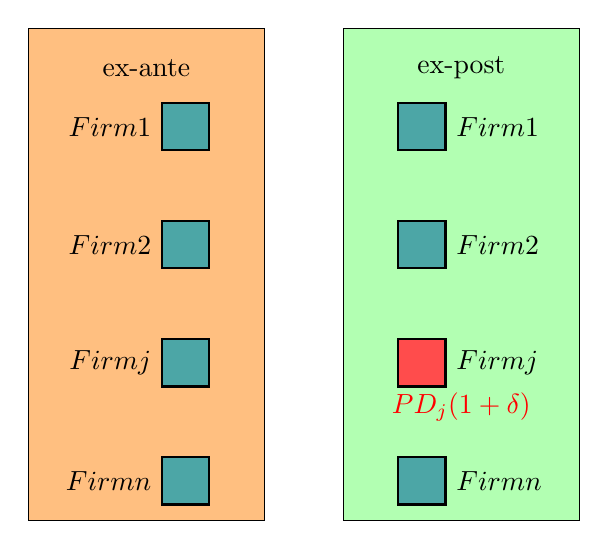
\begin{tikzpicture}
	[firm/.style={circle,draw=blue, fill=blue!70, thick,
				   inner sep=0pt, minimum size=6mm},
	 risk/.style={rectangle, inner sep=0pt, minimum size=6mm}]
	\draw[draw=black, fill=orange!50] (-2,-0.5) rectangle ++(3,6.25);
	\draw[draw=black, fill=green!30] (2,-0.5) rectangle ++(3,6.25);
	\node at (-0.5,5.25){ex-ante};
	\node at (3.5,5.25){ex-post};	 
	\node at (0,0)    [risk,draw=black, fill=teal!70, thick](rf4)
					  [label=left:$\text{Firm }n$]{};
	\node at (0,1.5)  [risk,draw=black, fill=teal!70,thick](rf3)
	                  [label=left:$\text{Firm }j$]{};
	\node at (0,3.0)  [risk,draw=black, fill=teal!70, thick](rf2)
				   	  [label=left:$\text{Firm }2$]{};
	\node at (0,4.5)  [risk,draw=black, fill=teal!70, thick](rf1)
	                  [label=left:$\text{Firm }1$]{};
	\node at (3,0)    [risk,draw=black, fill=teal!70, thick](rf4)
					  [label=right:$\text{Firm }n$]{};
	\node at (3,1.5)  [risk,draw=black, fill=red!70,thick](rf3)
	                  [label=right:$\text{Firm }j$]{};
    \node[red, below] at (3.5,1.25){$PD_j(1+\delta)$};
	\node at (3,3.0)  [risk,draw=black, fill=teal!70, thick](rf2)
				   	  [label=right:$\text{Firm }2$]{};
	\node at (3,4.5)  [risk,draw=black, fill=teal!70, thick](rf1)
	                  [label=right:$\text{Firm }1$]{};
\end{tikzpicture}
\end{center}
\end{frame}

\begin{frame} % Tarashev Borio Tsatsaronis
\frametitle{Tarashev, Borio, and Tsatsaronis (2010) portfolios}
\begin{center}
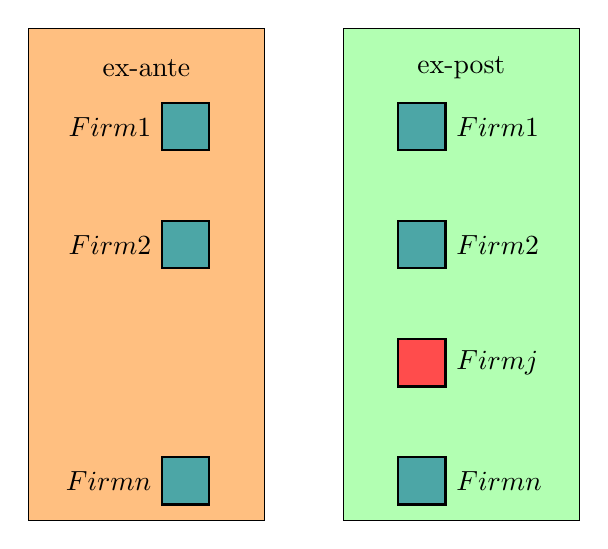
\begin{tikzpicture}
	[firm/.style={circle,draw=blue, fill=blue!70, thick,
				   inner sep=0pt, minimum size=6mm},
	 risk/.style={rectangle, inner sep=0pt, minimum size=6mm}]
	\draw[draw=black, fill=orange!50] (-2,-0.5) rectangle ++(3,6.25);
	\draw[draw=black, fill=green!30] (2,-0.5) rectangle ++(3,6.25);
	\node at (-0.5,5.25){ex-ante};
	\node at (3.5,5.25){ex-post};	 
	\node at (0,0)    [risk,draw=black, fill=teal!70, thick](rf4)
					  [label=left:$\text{Firm }n$]{};
%	\node at (0,1.5)  [risk,draw=black, fill=teal!70,thick](rf3)
%	                  [label=left:$\text{Firm }j$]{};
	\node at (0,3.0)  [risk,draw=black, fill=teal!70, thick](rf2)
				   	  [label=left:$\text{Firm }2$]{};
	\node at (0,4.5)  [risk,draw=black, fill=teal!70, thick](rf1)
	                  [label=left:$\text{Firm }1$]{};
	\node at (3,0)    [risk,draw=black, fill=teal!70, thick](rf4)
					  [label=right:$\text{Firm }n$]{};
	\node at (3,1.5)  [risk,draw=black, fill=red!70,thick](rf3)
	                  [label=right:$\text{Firm }j$]{};
%    \node[red, below] at (3.5,1.25){$PD_j(1+\delta)$};
	\node at (3,3.0)  [risk,draw=black, fill=teal!70, thick](rf2)
				   	  [label=right:$\text{Firm }2$]{};
	\node at (3,4.5)  [risk,draw=black, fill=teal!70, thick](rf1)
	                  [label=right:$\text{Firm }1$]{};
\end{tikzpicture}
\end{center}
\end{frame}

\begin{frame} % Chan-Lau
\frametitle{Chan-Lau (2010) portfolios}
\begin{center}
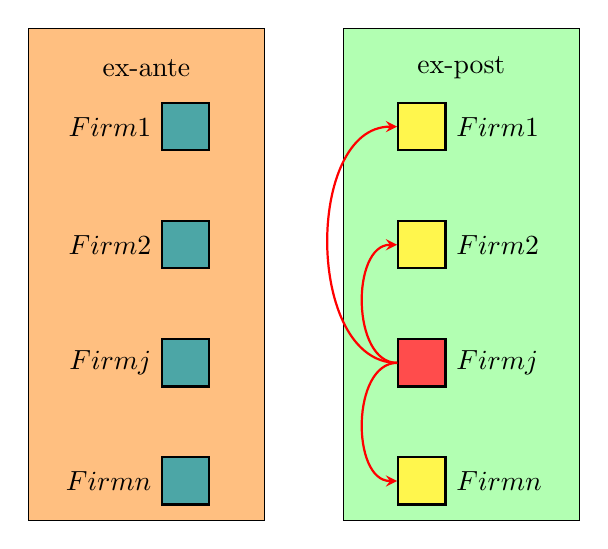
\begin{tikzpicture}
	[firm/.style={circle,draw=blue, fill=blue!70, thick,
				   inner sep=0pt, minimum size=6mm},
	 risk/.style={rectangle, inner sep=0pt, minimum size=6mm}]
	\draw[draw=black, fill=orange!50] (-2,-0.5) rectangle ++(3,6.25);
	\draw[draw=black, fill=green!30] (2,-0.5) rectangle ++(3,6.25);
	\node at (-0.5,5.25){ex-ante};
	\node at (3.5,5.25){ex-post};	 
	\node at (0,0)    [risk,draw=black, fill=teal!70, thick](rf4)
					  [label=left:$\text{Firm }n$]{};
	\node at (0,1.5)  [risk,draw=black, fill=teal!70,thick](rf3)
	                  [label=left:$\text{Firm }j$]{};
	\node at (0,3.0)  [risk,draw=black, fill=teal!70, thick](rf2)
				   	  [label=left:$\text{Firm }2$]{};
	\node at (0,4.5)  [risk,draw=black, fill=teal!70, thick](rf1)
	                  [label=left:$\text{Firm }1$]{};
	\node at (3,0)    [risk,draw=black, fill=yellow!70, thick](rf4)
					  [label=right:$\text{Firm }n$]{};
	\node at (3,1.5)  [risk,draw=black, fill=red!70,thick](rf3)
	                  [label=right:$\text{Firm }j$]{};
%    \node[red, below] at (3.5,1.25){$PD_j(1+\delta)$};
	\node at (3,3.0)  [risk,draw=black, fill=yellow!70, thick](rf2)
				   	  [label=right:$\text{Firm }2$]{};
	\node at (3,4.5)  [risk,draw=black, fill=yellow!70, thick](rf1)
	                  [label=right:$\text{Firm }1$]{};
	\draw[-stealth,red,thick]   (rf3) to [bend right = -90](rf1);
	\draw[-stealth,red,thick]   (rf3) to [bend right = -90](rf2);
	\draw[-stealth,red,thick]   (rf3) to [bend right = 90](rf4);                
\end{tikzpicture}
\end{center}
\end{frame}

\begin{frame} % Hands-on workshop: CoVaR
\Large{Hands-on-Exercise 3:\\
	Portfolio approaches}\\
	\vspace{1em}
	\Large{
	\begin{itemize}
		\item Huang, Zhou, and Zhu (2011)
		\item Tarashev, Borio, and Tsatsaronis (2010)
		\item Chan-Lau (2010)
	\end{itemize}
	}
	\vspace{1em}
\href{https://htmlpreview.github.io/?https://github.com/jchanlauimf/Systemic-Risk/blob/master/Portfolio Approach/Portfolio_Tutorial.html}{\beamergotobutton{Tutorial page}}		
\end{frame}

\section{Being practical: global systemically important banks (G-SIBs)}

\subsection{G-SIBs: Identification Methodology}

\begin{frame} % Indicators Based Approach (1)
\frametitle{Indicator-based Measurement Approach (1)}
	\begin{itemize}
		\item Global systemic importance
		\begin{itemize}
			\item (+) Impact of bank failure on global financial system and wider economy
			\item (-) Risk of a bank failure
		\end{itemize}
		\smallskip
		\item Subject to Higher Loss Absorbency (HLA) capital
		\smallskip
		\item Indicators approach
		\begin{itemize}
			\item Looks at negative externalities
			\item Reflects multiple dimensions of systemic risk
			\item Simple and robust methodology
		\end{itemize}
	\end{itemize}
\end{frame}

\begin{frame} % Indicators Based Approach (2)
\frametitle{Indicator-based Measurement Approach (2)}
	\begin{enumerate}
	\setbeamertemplate{enumerate items}[default]
		\item Size
		\medskip
		\item Interconnectedness
		\medskip
		\item Substitutability
		\medskip
		\item Cross-jurisdiction activity
		\medskip
		\item Complexity
	\end{enumerate}
\end{frame}

\begin{frame} % Indicators Based Approach (3)
\frametitle{Indicator-based Measurement Approach (3)}
\begin{center}
	\includegraphics[scale=0.38]{figures/figGSIBTable.eps}
\end{center}
\begin{flushleft}
	\tiny{Source: BCBS (2013)}
\end{flushleft}
\end{frame}

\begin{frame} % Indicators Based Approach (4)
\frametitle{Indicator-based Measurement Approach (4)}
For each bank
	\begin{itemize}
		\item Score of each indicator
		\[ \frac{\text{Individual bank amount}}{\text{Aggregate amount across banks}} \times 10000\] 
		\smallskip
		\item Category score is simple average over category
		\smallskip
		\item Overall score is simple average over five categories
	\end{itemize}

\end{frame}

\begin{frame} % Indicators Based Approach (5)
\frametitle{Indicator-based Measurement Approach (5)}
\begin{center}
Bucket thresholds, cut-off scores, and HLA requirement
\medskip
\vspace{1em}
	\begin{tabular}{ccc} 
	\hline \hline
	Bucket & Cut-off scores & HLA requirement \\
	& & \footnotesize{(common equity as percent of RWA)} \\
	\hline
	\\
	\rowcolor{Gray!20}5 & 530-629 & 3.5\% \\
	4 & 430-529 & 2.5\% \\
	\rowcolor{Gray!20}3 & 330-429 & 2.0\% \\
	2 & 230-329 & 1.5\% \\
	\rowcolor{Gray!20}1 & 130-229 & 1.0\% \\
	\\
	\hline
	\end{tabular}
\end{center}
\end{frame}

\begin{frame} % Indicators Based Approach (6)
\frametitle{Calibration of HLA requirement}
	\begin{itemize}
		\item Expected Impact Approach
		\begin{itemize}
			\item Impact of SIB failure greater than a non-SIB reference bank
			\smallskip
			\item Set $P(SIB) = P(\text{Ref Bank})/\text{Factor}$, where $\text{Factor}>1$
			\smallskip
			\item Factor = cost of SIB failure relative to reference bank
			\smallskip
			\item With $P(SIB)$ use empirical distribution or Merton model to determine HLA 
		\end{itemize}
		\smallskip
		\item Long run net economic costs of higher capital requirements
		\smallskip
		\item Too-big-to-Fail funding subsidies 
	\end{itemize}
\end{frame}

\begin{frame} % Expected Impact Approach
\frametitle{Expected Impact Approach}
\begin{center}
	\includegraphics[scale=0.40]{figures/figHLACalibration.eps}
\end{center}
\end{frame}

\begin{frame} % Indicators Based Approach (7)
\frametitle{FSB 2016 G-SIBs}
\begin{center}
	\includegraphics[scale=0.35]{figures/figGSIBBucketsFirms.eps}
\end{center}
\begin{flushleft}
	\tiny{Source: FSB (2016)}
\end{flushleft}
\end{frame}

\begin{frame} % Proposed revisions to Methodology 1
\frametitle{Proposed Revisions to Methodology (1)}
\begin{center}
	\includegraphics[scale=0.5]{figures/figGSIBUpdateTable.eps}
\end{center}
\begin{flushleft}
	\tiny{Source: BCBS (2017)}
\end{flushleft}
\end{frame}

\begin{frame} % Proposed revisions to Methodology 2
\frametitle{Proposed Revisions to Methodology (2)}
\begin{center}
	\includegraphics[scale=0.4]{figures/figGSIBUpdateImpact.eps}
\end{center}
\begin{flushleft}
	\tiny{Source: BCBS (2017)}
\end{flushleft}
\end{frame}

\section{New directions}

\subsection{Systemic communities}

\begin{frame} % Systemic communities
\frametitle{Systemic communities (1)}
\begin{itemize}
	\item Cross-section systemic risk
		\begin{itemize}
			\item Too-connected-to-fail (TCTF)
			\item Too-important-to-fail (TITF)
		\end{itemize}
	\smallskip
	\item TCTF captured with centrality measures
	\smallskip
	\item Communities capture TITF
		\begin{itemize}
			\item Group of (fully or not) connected firms
			\item Failure of one firm affects community
		\end{itemize}
	\item Centrality and community analysis are complementary
\end{itemize}
\end{frame}

\begin{frame} % Systemic communities
\frametitle{Systemic communities (2)}
\begin{itemize}
	\item Community detection 
		\begin{itemize}
			\item Active area of research 
			\item Physics
			\item Biology
			\item Computer science
			\item Computational Social Sciences
		\end{itemize}
	\smallskip
	\item Methods applied in finance/economics
		\begin{itemize}
			\item Clique percolation
			\item Edge betweeness
			\item Infomap
		\end{itemize}
\end{itemize}
\end{frame}

\begin{frame} % Clique percolation
\frametitle{Systemic communities (3): clique percolation method}
\begin{center}
	\includegraphics[scale=0.65]{figures/figCPM01.eps}
\end{center}
\tiny{Source: Derenyi, Palla, and Vicsek (2005) }
\end{frame}

\begin{frame} % Mandatory FSAP 2013
\frametitle{Systemic communities (4): IMF Mandatory FSSA 2013}
\begin{center}
	\includegraphics[scale=0.4]{figures/figMandatoryFSAP.eps}
\end{center}
\tiny{Source: Demekas et al (2013)}
\end{frame}

\begin{frame} % Infomap algorithm
\frametitle{Systemic communities (5): Infomap algorithm}
\begin{center}
	\includegraphics[scale=0.45]{figures/figInfoMap.eps}
\end{center}
\tiny{Source: Rosvall and Bergstrom (2008); Bohlin et al (2014)}
\end{frame}

\begin{frame} % Infomap algorithm
\frametitle{Systemic communities (6): edge betweenness}
\begin{center}
	\includegraphics[scale=0.55]{figures/figEdgeBetweeness.eps}
\end{center}
\tiny{Source: Meghanathan, N. 2016. A greedy algorithm for neighborhood overlap-based community detection. \textit{Algorithms}} 9.
\end{frame}

\begin{frame} % Systemic communities in a VAR decomposition network
\frametitle{Systemic communities (7): global financial network}
\begin{center}%
	\includegraphics[scale=0.35]{figures/figCommunitiesAlgorithms.eps}
\end{center}
\tiny{Source: Chan-Lau (2017)}
\end{frame}

\subsection{Agent-based network models} 

\begin{frame} % Agent-based networks (1)
\begin{center}
\frametitle{Agent-based networks (1)}
	\includegraphics[scale=0.30]{figures/figABBABankFlowChart.eps}
\end{center}
\tiny{Source: Chan-Lau (2017)}
\end{frame}

\begin{frame} % Agent-based networks (2)
\begin{center}
\frametitle{Agent-based networks (2)}
	\includegraphics[scale=0.45]{figures/figABBA01.eps}
\end{center}
\tiny{Source: Chan-Lau (2017)}
\end{frame}

\begin{frame} % Agent-based networks (3)
\begin{center}
\frametitle{Agent-based networks (3)}
	\includegraphics[scale=0.35]{figures/figABBADegrees.eps}
\end{center}
\tiny{Source: Chan-Lau (2017)}
\end{frame}

\section{Summary}

\begin{frame} % Summary
\frametitle{Summary}
\begin{itemize}
	\item Financial systems are networks
	\smallskip
	\item Networks construction
	\begin{itemize}
		\item Direct exposures
		\item Market-based measures
	\end{itemize}
	\smallskip
	\item Analytical methods
	\begin{itemize}
		\item Rapid development going on
		\item Useful and easy to implement
			\begin{itemize}
				\item Balance-sheet network analysis
				\item CoVaR (and CoRisk)
				\item Portfolio approaches
			\end{itemize}
	\end{itemize}
	\smallskip
	\item New approaches finding their way into policy
	\smallskip
	\item Self-study: keep up with analytics to remain relevant!
\end{itemize}
\end{frame}

\begin{frame} % Thank You
	\centering
	\Huge{Thank You}
\end{frame}

\section*{References}

\begin{frame} % References (1)
\frametitle{References (1)}
\scriptsize{\textbf{Conceptual Overview}}
\tiny{
\begin{itemize}
	\item Bookstaber, R., Kenett,D. 2016 Looking deeper, seeing more: a multilayer map of the financial system. OFR Brief Series 16-06.
	\item Borio, C. 2001. Towards a macroprudential framework for financial supervision and regulation. BIS WP No. 128.
	\item Brunnermeier, M., Pedersen, L. 2009. Market liquidity and funding liquidity. \textit{Review of Financial Studies} 22.
	\item Zhao, Z., Zhang, W., Shi, S. 2013. Common asset holdings and systemic risk of financial network. \textit{Procedia Computer Science} 17.
\end{itemize}
}
\vspace{1ex}
\scriptsize{\textbf{Direct Exposure Methods}}
\tiny{
\begin{itemize}
	\item Bardoscia, M., Battiston, S., Caccioli, F., Caldarelli, G. 2015. DebtRank: a microscopic foundation for shock propagation. PLOS One. June 19.
	\item Bargigli, L., di Iasio, G., Infante, L., Pierobon, F. 2015. The multiplex structure of interbank networks. \textit{Quantitative Finance}.
	\item Chan-Lau, J.A. 2010. Network analysis model. User's guide. Internal document. Banco Central de Chile.
	\item Espinosa, M., Sole, J. 2010. Cross-border financial surveillance: a network perspective. IMF  WP 10/105.
	\item Eisenberg, L., Noe, T.H. 2001. Systemic risk in financial systems. \textit{Management Science} 47. 
	\item Furfine, C. 2003. Interbank exposures: quantifying the risk of contagion. \textit{J. of Money, Credit and Banking} 35.
	\item Jo, J.-H. 2012. Managing systemic risk from the perspective of the financial network under macroeconomic distress. FSI Award 2012 Winning Paper. Financial Stability Institute, Basel.
	\item Sun, A., Chan-Lau, J.A. 2017. Financial networks and interconnectedness in an advanced emerging market economy. \textit{Quantitative Finance}, in print.
	\item Upper, C. 2011. Simulation methods to assess the danger of contagion in interbank markets. \textit{J. of Financial Stability} 7.
\end{itemize}
}
\end{frame}

\begin{frame} % References (2)
\frametitle{References (2)}
\scriptsize{\textbf{Market-based Methods}}
\tiny{
\begin{itemize}
	\item Adrian, T., Brunnermeier, M. 2016. CoVaR. \textit{American Economic Review} 106.
	\item Barigozzi, M., Brownless, C.T. 2016. NETS: Network estimation for time series. Mimeo, LSE and U. Pompeu Fabra.
	\item Billio, M. Getmansky, M., Lo, A., Pellizon, L. 2012. Econometric measures of connectedness and systemic risk in the finance and insurance sectors. \textit{J. of Financial Economics} 104.
	\item Chan-Lau, J.A. 2009. Default risk codependence in the global financial system: was the Bear Stearns bailout justified? In Gregoriu, G. \textit{The Banking Crisis Handbook}. John Wiley and Sons
	\item Chan-Lau, J.A. 2017. Variance decomposition networks: potential pitfalls and a simple solution. IMF WP 17/107.
	\item Chan-Lau, J.A., Chuang, C., Duan, J.-C., Sun, W. 2017. Financial network and systemic risk via forward-looking partial default correlations. Mimeo. National University of Singapore.
	\item Craig, B., Saldias, M., 2016. Spatial dependence and data-driven networks of international banks. IMF WP 16/184.
	\item Diebold, F., Yilmaz, M. 2014. On the network topology of variance decompositions: measuring the connectedness of financial firms. \textit{J. of Econometrics} 182.
	\item Kenett, D., Tumminello, M., Madi, A., Gur-Gershgoren, G., Mantegna, R., Ben-Jacob, E. 2010. Dominating clasp of the financial sector revealed by partial correlation analysis of the stock market. PLOS One December 20.
	\item Klossner, S., Wagner, S. 2014. Exploring all VAR orderings for calculating spillovers? Yes, we can! A note on Diebold and Yilmaz. \textit{J. of Applied Econometrics} 29.
\end{itemize}
}
\end{frame}

\begin{frame} % References (3)
\frametitle{References (3)}
\scriptsize{\textbf{The Portfolio Approach}}
\tiny{
\begin{itemize}
	\item Tarashev, N., Borio, C., Tsatsaronis, K. 2010. Attributing systemic risk to individual institutions. BIS WPs No. 308.
	\item Chan-Lau, J.A. 2010. Regulatory Capital Charges for Too-Connected-to-Fail Institutions: A Practical Proposal. \textit{Financial markets, Institutions, and Instruments} 19 (Lead Article).
	\item Chan-Lau, J.A. 2013. \textit{Systemic Risk Assessment and Oversight}. Risk Books. London.
	\item Huang, X., Zhou, H., Zhu, H. 2011. Systemic risk contributions. FEDS WP 2011-08. Board of Governors of the Federal Reserve.
\end{itemize}
}
\vspace{1ex}
\scriptsize{\textbf{Systemic communities}}
\tiny{
\begin{itemize}
	\item Bohlin, L., Edler, D., Lancichinetti, A., Rosvall, M. 2014. Community detection and visualization of networks with the map equation framework. Mimeo.
	\item Chan-Lau, J.A. 2017. Systemic centrality and systemic communities in financial networks. Mimeo, IMF.
	\item Demekas, D., Chan-Lau, J.A., Rendak, N.,Ohnsorge, F., Youssef, K., Caceres, C., Tintchev, K. 2013. Mandatory financial stability assessments under the financial sector assessment program: update. IMF.
	\item Derenyi, I., Palla, G., Vicsek, T. 2005. Clique percolation in random networks. \textit{Physics Review Letters} 94.	
	\item Girvan, M., Newman, M.E.J. 2002. Community structure in social and biological networks. \textit{Proc. of the National Academy of Sciences} 99.
	\item Palla, G., Farkas, I.J., Vicsek, T. 2005. Uncovering the overlapping community structure of complex networks in nature and society. \textit{Nature} 435.
	\item Rosvall, M., Bertstrom, C. 2008. Maps of random walks on complex networks reveal community structure. \textit{Proc. of the National Academy of Sciences} 105.
\end{itemize}
}
\end{frame}

\begin{frame} % References (4)
\frametitle{References (4)}
\scriptsize{\textbf{Agent-based models}}
\tiny{
\begin{itemize}
	\item Chan-Lau, J.A. 2014. Regulatory requirements and their implications for bank solvency. Mimeo. IMF and NUS.
	\item Chan-Lau, J.A. 2017. ABBA: an Agent-based model of the banking system. IMF WP/17/136.
	\item Halaj, G., Kok C.. 2014. Modeling emergence of the interbank networks. ECB WP No. 1646.
	\item Liu, A., Paddrik, M., Yang, S., Zhang, X. 2016. Interbank contagion: an agent-based model approach to endogenously formed networks. OFR WP 16-15.
	\item Turrell, A. 2016. Agent-based models: understanding the economy from the bottom up. Quarterly bulletin Q4. Bank of England. 
\end{itemize}
}
\vspace{1ex}
\scriptsize{\textbf{Global systemic institutions}}
\tiny{
\begin{itemize}
\item BCBS. 2012. A framework for dealing with domestic systemically important banks. Basel.
\item BCBS. 2017. Global systemically important banks - revised assessment framework. Consultative document. Basel.
\item FSB. 2016. 2016 list of global systemicallly important banks (G-SIBs).
\item IAIS. 2016. Global systemically important insurers: updated assessment methodology. 
\end{itemize}
}
\vspace{1ex}
\scriptsize{\textbf{Other useful references}}
\tiny{
\begin{itemize}
	\item Bisias, D., Flood, M., Lo, A.W., S. Valavanis. 2012. A survey of systemic risk analytics. OFR WP 0001.
	\item Gai, P. 2016. \textit{Systemic Risk: the dynamics of modern financial systems.} Oxford University Press.
	\item Glasserman, P., Young, H.P. 2016. Contagion in financial networks. \textit{J. of Economic Literature} 54.
	\item Hamill, L., Gilbert, N. 2016. \textit{Agent-based modelling in economics}. John Wiley and Sons.
\end{itemize}
}
\end{frame}

\end{document}

